\documentclass[10pt]{book}
\usepackage[T1]{fontenc}
\usepackage[utf8]{inputenc}
\usepackage[italian]{babel}
\usepackage[document]{ragged2e}
\usepackage{microtype}
\usepackage{notomath}
\usepackage{CharisSIL}
\usepackage[all]{nowidow}
\usepackage{graphicx}
\usepackage{svg}
\usepackage[pdfa]{hyperref}
\usepackage{color}
\usepackage{setspace}
\usepackage{parskip}
\usepackage[a4paper, inner=4.0cm, outer=5.0cm]{geometry}
\usepackage{listings}
\definecolor{dkgreen}{rgb}{0.1,0.5,0.1}
\definecolor{greengray}{rgb}{0.517,0.761,0.404}
\definecolor{orange}{rgb}{0.717,0.274,0.105}
\definecolor{blue}{rgb}{0.164,0.317,0.600}
\definecolor{background}{rgb}{0.990,0.990,0.990}
\lstset {
	frame=lrtb,
	language=java,
	aboveskip=0.7cm,
	belowskip=0.2cm,
	showstringspaces=false,
	columns=flexible,
	basicstyle={\small\ttfamily},
	numbers=none,
	backgroundcolor=\color{background},
	numberstyle=\tiny\color{dkgreen},
	keywordstyle=\color{blue},
	commentstyle=\color{greengray},
	stringstyle=\color{orange},
	breaklines=true,
	breakatwhitespace=true,
	tabsize=3
}

\newtheorem{thm}{Teorema}
\setlength{\tabcolsep}{0.5em} % for the horizontal padding
{\renewcommand{\arraystretch}{1.35}% for the vertical padding

\usepackage{fancyhdr}


\pagestyle{fancy}
\fancyhf{}
\fancyhead[LE,RO]{\leftmark}
%\fancyhead[RE,LO]{Programmazione Avanzata}
%\fancyfoot[CE,CO]{\leftmark}
\fancyfoot[LE,RO]{\thepage}

\renewcommand{\headrulewidth}{1pt}
%\renewcommand{\footrulewidth}{1pt}

\usepackage{titlesec}
\titleformat{\part}[display]
{\Huge\bfseries}{}{10pt}{\center{ Parte \thepart\ \ \\ \ \ }}
%\titleformat{\chapter}[display]
%{\huge\bfseries}{}{0pt}{\thechapter\ \ \--\ \ }
\titleformat{\section}[display]
{\Large\bfseries}{}{0pt}{\medskip\thesection\ \ \--\ \ }
\titleformat{\subsection}[display]
{\large\bfseries}{}{0pt}{\medskip\thesubsection\ \ \--\ \ }

\begin{document}
\setmonofont[Scale=.85]{Fira Code Retina}


\begin{titlepage}
        \begin{center}
                \Large
                \textbf{UNIVERSITÀ DEGLI STUDI DI TRIESTE}

                \par\noindent\rule{\textwidth}{0.8pt}
                \vspace*{0.6cm}

                \large
                \emph{Marco Sgobino}

                \large
                \vspace*{0.6cm}

                \Large Dispense del corso di
                \vspace*{0.6cm}

                \Huge
                \textsc{Complessità e Crittografia}
                \vspace*{.1cm}

                %\large 
                %\emph{sezione intermedia}

                \vspace*{2cm}

                \begin{center}
                        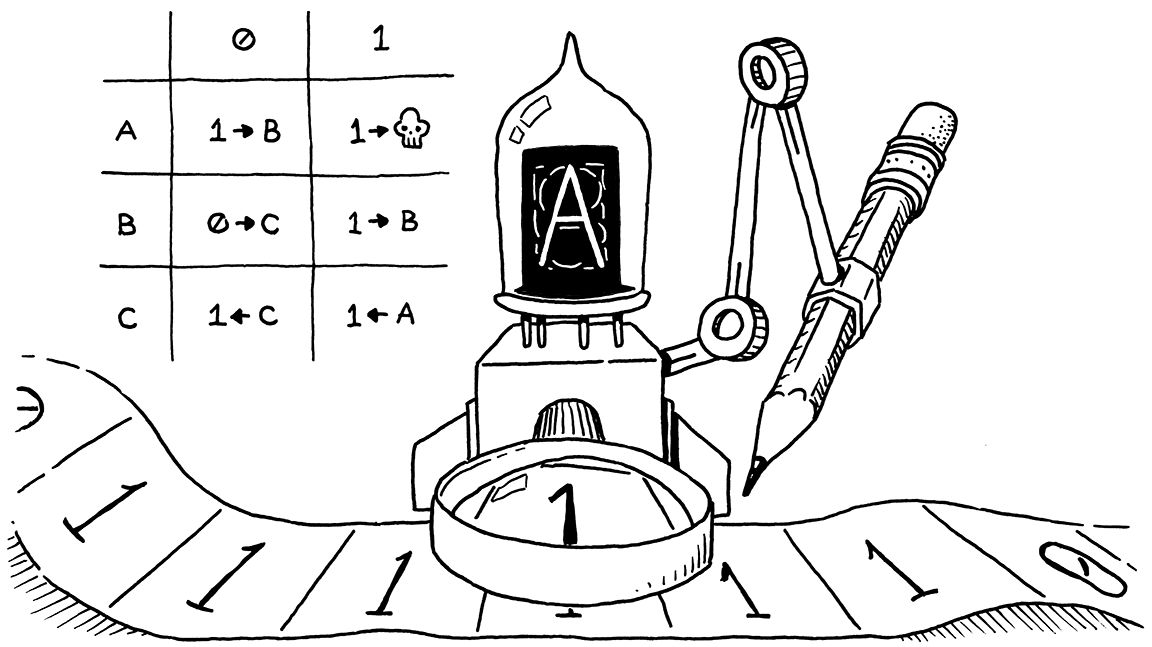
\includegraphics[width=.9\textwidth, keepaspectratio]{./pics/turing-machine-titlepage.png}
                \end{center}

                \vfill

                \par\noindent\rule{\textwidth}{0.8pt}
                \vspace*{0.6cm}
                \large
                \emph{Anno Accademico 2021-2022}

        \end{center}
\end{titlepage}


\setstretch{1.35}
\setlength{\headsep}{30pt}
\setlength{\footskip}{40pt}
\setlength{\marginparsep}{20pt}
\setlength{\marginparwidth}{60pt}

%\title{Complessità}
%\author{Marco Sgobino}
%\maketitle
\tableofcontents

%\part{Complessità}
\chapter{La macchina di Turing}
\section{Descrizione della macchina}

Una \emph{macchina di Turing} è una macchina che è descritta da un insieme di
\emph{simboli} $\Gamma = \{\alpha, \beta, \gamma, \delta, \dots\}$ \emph{finito} e da
un insieme di \emph{stati} $\mathcal{Q} = \{q_1, q_2, \dots, q_n\}$ anch'esso
\emph{finito}. La macchina di Turing dispone di un nastro di memoria \emph{potenzialmente
illimitato} a destra e a sinistra, avente delle celle contenenti i simboli;
essa identifica il simbolo nella posizione dove la
\emph{testina} della macchina è collocata sul nastro. Ad ogni iterazione della
macchina di Turing viene letto il simbolo, e a seconda dello stato $q_i$, viene
intrapresa un'azione fra le $3$ seguenti:
\begin{itemize}
    \item spostamento della testina a destra;
    \item spostamento della testina a sinistra;
    \item riscrittura del simbolo sotto la testina con uno qualsiasi
        appartenente all'alfabeto di simboli.
\end{itemize}

Nello specifico, una macchina di Turing è univocamente identificata dalla sua
\emph{matrice di transizione} $\delta  : \mathcal Q \times \Gamma \rightarrow
\mathcal Q \times (\Gamma \cup \{L,R\})$\footnote{In talune circostanze, è
possibile trovare una definizione differente, cioè $$\delta  : \mathcal Q \times
\Gamma \rightarrow \mathcal Q \times \Gamma \times \{L,R\};$$ in altre parole, è
una macchina che \emph{si muove sempre sul nastro,} poiché per ogni stato è
sempre definito un movimento. Per questo tipo di macchina, sono necessarie
diverse regole d'ingaggio, e i programmi in essa costruiti saranno radicalmente
differenti. La differenza fra i due modelli rappresenta un'evidenza della
versatilità della macchina di Turing.}, dove i simboli $L$ ed $R$ sono
rappresentativi dell'azione di spostarsi, rispettivamente, a sinistra e a
destra del nastro di memoria. La matrice di transizione lega, dunque, ciascuno
stato al simbolo collocato immediatamente sotto alla testina nel nastro di
memoria, stabilendo in maniera univoca l'azione da intraprendere. Si può dire
dunque che la matrice di transizione fornisce alla macchina di Turing l'elenco
delle possibili azioni da intraprendere, alla lettura di un simbolo sulla cella
corrente, a seconda dello stato in cui si trova. L'insieme delle azioni che la
macchina di Turing compie è quindi la realizzazione del programma stesso,
quello che nei termini del modello RAM si sarebbe detto essere la sequenza di
istruzioni elementari.

Una macchina di Turing può anche essere accompagnata da un alfabeto
\emph{ausiliario}, ovverosia un alfabeto $\mathcal V$ comprendente simboli
simili a quelli di $\Gamma$, ma che vengono utilizzati qualora la macchina di
Turing avesse \emph{già processato} la cella in questione (i simboli ausiliari
sono ``simili'' a quelli dell'alfabeto tradizionale, ma hanno una differenza
che ne permette il riconoscimento). Tipicamente, l'utilizzo dell'alfabeto
ausiliario è importante nel caso specifico in cui si adoperino procedure per le
quali è utile ricordare se una cella sia già stata in precedenza processata
dalla macchina di Turing, oppure no \-- in ogni caso, l'alfabeto ausiliario è
meramente un sussidio che permette una semplificazione della procedura o aiuta
ad interpretare il comportamento della macchina, non è in nessun modo un
qualsivoglia tipo di estensione della macchina di Turing. Come sarà mostrato in
seguito, ciascuna altra possibile definizione di macchina di Turing è, dal
punto di vista della potenza computazione, del tutto equivalente alla
definizione già data sopra.


\begin{table}[ht]
\centering
\begin{tabular}{c|cccc}
    & $q_1$ & $q_2$ & $\cdots$ & $q_n$ \\
    \hline
$\alpha$ & $\beta/q_2$ & $\gamma/q_2$ & $\cdots$ & \\
$\beta$ & $L/q_1$ & $\gamma/q_3$ & $\cdots$ & \\
$\gamma$ & $\gamma/q_3$ & $R/q_2$ & $\cdots$ & \\
$\vdots$ & $\vdots$ & $\vdots$ & $\ddots$ &    
\end{tabular}
\caption{Possibile matrice di transizione per una macchina di Turing. Le righe
corrispondono ai simboli dell'alfabeto $\Gamma$, mentre le colonne sono
corrispondenti ai singoli stati dell'insieme $\mathcal
Q$. Ogni elemento della tabella indica il simbolo da scrivere/stato in cui la
macchina dovrà trovarsi al passo successivo,}\label{tab:matriceTransizione}
\end{table}
\bigskip


Diversamente dal modello RAM, la quantità di memoria destinata ad ogni cella è
\emph{limitata}, poiché vi può essere collocato soltanto un numero finito di
simboli, quelli appunto dell'insieme $\Gamma$. Ciononostante, la macchina di
Turing si presta meglio alla trattazione di stringhe, poiché i simboli possono
rappresentare qualsivoglia tipologia di entità astratta, mentre per il modello
RAM si avrebbe necessità di una codifica fra numeri reali e simboli da
trattare. Non vi è più dunque la limitazione imposta dal fatto che all'interno
di una cella possa risiedere esclusivamente un numero naturale, non importa
quanto grande sia; nella macchina di Turing le celle possono contenere simboli
di qualsiasi natura essi siano. Lo ``svantaggio'', tuttavia, è che all'interno di
ogni cella non può essere contenuta una quantità \emph{arbitraria} di
informazione, come invece avveniva per il modello RAM, che faceva uso dei
numeri naturali.

Tipicamente, assieme all'alfabeto che definisce una macchina di Turing viene definito
un sottoinsieme sigma di \emph{simboli di input}, $\Sigma \subset \Gamma$, in
concomitanza al quale viene definito un simbolo vuoto, \emph{blank}, $b \in
\Gamma - \Sigma$. Il simbolo $b$ incarna dunque l'idea di \emph{cella
vuota} \-- si pensi infatti al valore che una cella di memoria primaria
qualsiasi di un computer reale avrebbe, al momento immediatamente successivo
all'accensione: essa risulterebbe posta allo zero logico, di fatto non
conterrebbe alcun valore d'interesse, dato che essa non è ancora stata
``toccata'' dall'esecuzione di alcun programma. Il simbolo \emph{blank} sta a
significare proprio questo, ed è l'equivalente del valore `zero' del modello
RAM, dove all'avvio del programma ogni cella di memoria fuorché quelle
contenenti i valori di ingresso contiene il numero reale $0$. 

Ricapitolando, ogni macchina di Turing viene univocamente definita da:
\begin{itemize}
    \item un insieme finito di simboli $\Gamma$ \--- essi comprendono sia i
        simboli di input $\Sigma$ che il simbolo \emph{blank} $b$;
    \item un insieme finito di stati $\mathcal Q$;
    \item una funzione (matrice) di transizione $\delta  : \mathcal Q \times
        \Gamma \rightarrow \mathcal Q \times (\Gamma \cup \{L,R\})$.
\end{itemize}

Una diversa maniera per definire una macchina di Turing è tramite la
\emph{quaterna} o \emph{quadrupla} $q_i, s_j, \alpha, q_k$, dove $q_i$ è lo
\emph{stato in cui si trova la macchina}, $s_j$ è il \emph{simbolo letto dalla
testina}, $\alpha$ è il \emph{simbolo scritto nella matrice di transizione} e
$q_k$ è lo \emph{stato successivo} in cui la macchina di Turing si troverà al
termine dell'esecuzione di $\alpha$. In particolare, l'operazione che la
macchina di Turing effettua dipende dal simbolo $\alpha$ scritto nella matrice
di transizione:
\begin{itemize}
    \item se $\alpha = s_i$, sostituisci il simbolo $s_j$ con $s_i$;
    \item se $\alpha = R$, muovi la testina a destra;
    \item se $\alpha = L$, muovi la testina a sinistra.
\end{itemize}

In parole povere, una macchina di Turing può sovrascrivere un simbolo presente
sulla cella con un altro presente nel suo alfabeto, $\Gamma$, può spostare la
testina di un'unità a destra, e può fare altrettanto a sinistra.

Resta da scogliere il nodo relativo alla terminazione della macchina di Turing.
Nel modello RAM, la terminazione avveniva qualora le istruzioni si fossero
esaurite, o più precisamente qualora l'indice dell'istruzione successiva fosse
quello di un'istruzione assente nella sequenza che definisce la procedura. In
assenza del concetto di ``istruzione'', secondo quale regole dovrebbe terminare
una macchina di Turing? 

Lo \emph{stop} della computazione di una macchina di Turing avviene qualora la
coppia $q_i, s_j$ \textbf{non} sia presente nella matrice di transizione. Nel
caso di una coppia simbolo\----stato non presente nella matrice di transizione,
la macchina di Turing avrà terminazione, e vi sarà il riconoscimento del valore
finale di computazione, espresso similmente al caso del modello RAM con una
convenzione che permetta di identificare il valore finale del risultato della
computazione.

Se lo stop della computazione è stato chiarito, ora resta da definire il metodo
con cui andremo a recuperare il valore finale della computazione.
Convenzionalmente, l'esito di una macchina di Turing è una particolare
configurazione di memoria dello stato finale. Si è infatti scelto che
il risultato $f(x)$ sia da leggersi come il numero totale di occorrenze di $1$
(meno una) sul nastro nella configurazione iniziale, se la computazione è
andata a convergenza \-- indefinito altrimenti. La sequenza di occorrenze del
simbolo $1$ è delimitata dal carattere \emph{blank}. Quindi vi saranno $f(x) +
1$ simboli \textquotesingle1\textquotesingle, e pertanto sarà da contare un
simbolo \textquotesingle1\textquotesingle\ in meno (lo
\textquotesingle0\textquotesingle\   sarà indicato con la presenza di un
singolo simbolo \textquotesingle1\textquotesingle). Per quanto invece riguarda
i risultati di tipo \emph{vettoriale}, cioè del tipo $f(x_1,x_2,\dots,x_n)$,
ebbene sarà sufficiente costruire $n$ ``quadrati'' in cui racchiudere gli $x+1$
simboli $1$, ciascuno delimitato dal simbolo \emph{b}. In altre parole, la
situazione è quella descritta dalla Figura~\ref{fig:mdtRisultato}.

\begin{figure}[b]
    \centering
    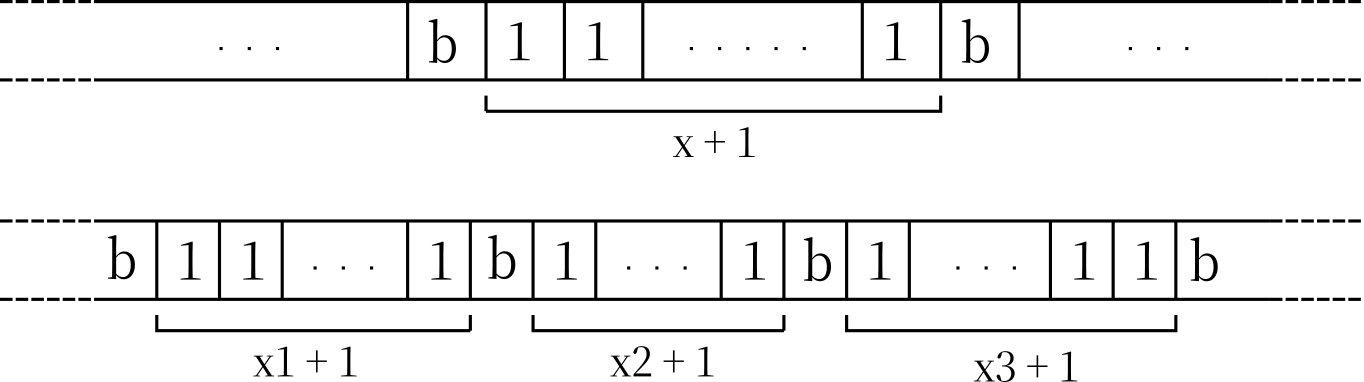
\includegraphics[ width=1.0\linewidth, height=\textheight, keepaspectratio]{./pics/mdtRisultato.png}
    \caption{Risultato singolo (sopra) e \emph{vettoriale} (sotto) di una macchina di Turing.}
    \label{fig:mdtRisultato}
\end{figure}



Per via dell'utilizzo tramite la matrice di transizione è particolarmente
difficile programmare sulla macchina di Turing~\--~questo è principalmente
dovuto al fatto che la macchina di Turing è una macchina `a stati', dove non vi è
un insieme di istruzioni da applicare direttamente, ma è necessario determinare
prima di tutto la matrice di transizione relativa a ciò che bisogna calcolare,
stato per stato e simbolo per simbolo.

Una macchina di Turing, non importa come sia stata definita, può essere
adoperata sostanzialmente per compiere $3$ operazioni:
\begin{enumerate}
    \item per il \emph{calcolo} di una funzione \--- la macchina di Turing è
        intesa come \emph{calcolatore}, e lo scopo è quello di calcolare una
        funzione $f: \mathbb{N}^n \rightarrow \mathbb{N}$. In questo caso, la
        macchina di Turing risulta essere meno efficiente del modello RAM, per
        via dell'assenza del comodo sistema di istruzioni presente in quest
        ultimo;
    \item per il \emph{riconoscimento} di una stringa \--- la macchina di
        Turing è intesa come \emph{accettore}. In questo contesto la MdT è
        molto più efficiente del modello RAM, poiché non è richiesta la
        codifica da numeri naturali a simboli;
    \item per la \emph{decisione} di un predicato \--- la macchina di Turing è
        intesa come \emph{decisore}.
\end{enumerate}

\subsection{Equivalenza fra macchina di Turing e $\mathcal R$}

Un importante teorema definisce l'equivalenza della macchina di Turing (avente
insieme delle funzioni computabili $\mathcal{TC}$ all'insieme delle funzioni
parziali ricorsive $\mathcal R$, e lo lega indissolubilmente all'insieme delle
funzioni computabili dal modello RAM $\mathcal C$.

\begin{thm}{dell'equivalenza della macchina di Turing all'insieme $\mathcal R$
    delle funzioni parziali ricorsive}
    $$\mathcal R \equiv \mathcal {TC} \equiv \mathcal C$$
\end{thm}

\textsc{Dimostrazione} \---- Un possibile spunto di dimostrazione di $\mathcal {TC} \subseteq \mathcal R$ si
ha grazie al fatto che la configurazione e lo stato della MdT durante la
computazione possono essere codificati da un numero naturale; le operazioni
sulla macchina sono rappresentate da funzioni ricorsive su questi numeri. Il
viceversa è invece mostrabile tenendo conto che si può verificare che
$\mathcal{TC}$ contiene le funzioni di base ed è chiusa rispetto a sostituzione,
ricorsione e minimazione illimitata.

\subsection{Macchina di Turing per il calcolo della somma}

Supponiamo di voler fare la somma fra due numeri interi naturali, $x$ ed $y$.
In questo caso, la macchina di Turing dovrebbe calcolare la funzione $f(x,y) =
x + y$. Per fare ciò, costruiremo gli elementi fondamentali della macchina di
Turing. In particolare, avremo che l'alfabeto di simboli $\Gamma = \{0, 1,
b\}$, cioè avremo bisogno esclusivamente di $2$ simboli eccezion fatta per il
simbolo \emph{blank}, mentre invece faremo uso di $3$ stati $\mathcal Q =
\{q_1, q_2, q_3\}$. Lo stato iniziale è lo stato $q_1$, mentre lo stato finale
è $q_3$. Resta ora da definire la matrice di transizione. Uno fra i tanti modi
di definirla è il seguente (faremo uso delle quadruple),


\begin{table}[ht]
\centering
\begin{tabular}{cccc}
    $q_1$ & $1$ & $b$ & $q_1$\\
    $q_1$ & $b$ & $R$ & $q_2$\\
    $q_2$ & $1$ & $b$ & $q_3$\\
    $q_2$ & $b$ & $R$ & $q_2$

\end{tabular}
\caption{Matrice di transizione per la macchina di Turing che calcola $f(x,y) =
x + y$.}\label{tab:mdtSomma}
\end{table}
\bigskip

L'idea è quella di togliere due simboli $1$, di modo che gli $1$ rimanenti
corrispondano al valore del risultato finale. Infatti, provando a calcolare
$f(2, 1) = 3$ avremo che

\begin{table}[ht]
\centering
\begin{tabular}{cccccccc}
   $q_1$&     &     &     &     &     &     &     \\
    $1$ & $1$ & $1$ & $b$ & $1$ & $1$ & $b$ & $b$ \\
   $q_1$&     &     &     &     &     &     &     \\
    $b$ & $1$ & $1$ & $b$ & $1$ & $1$ & $b$ & $b$ \\
        &$q_2$&     &     &     &     &     &     \\
    $b$ & $1$ & $1$ & $b$ & $1$ & $1$ & $b$ & $b$ \\
        &     &$q_3$&     &     &     &     &     \\
    $b$ & $b$ & $1$ & $b$ & $1$ & $1$ & $b$ & $b$
\end{tabular}
\end{table}
\bigskip

ed il numero finale di simboli $1$ corrisponde proprio al valore della somma,
$2 + 1 = 3$.

Possiamo anche costruire un grafo della macchina di cui sopra, mostrato in
Figura~\ref{fig:mdtSomma}.


\begin{figure}[b]
    \centering
    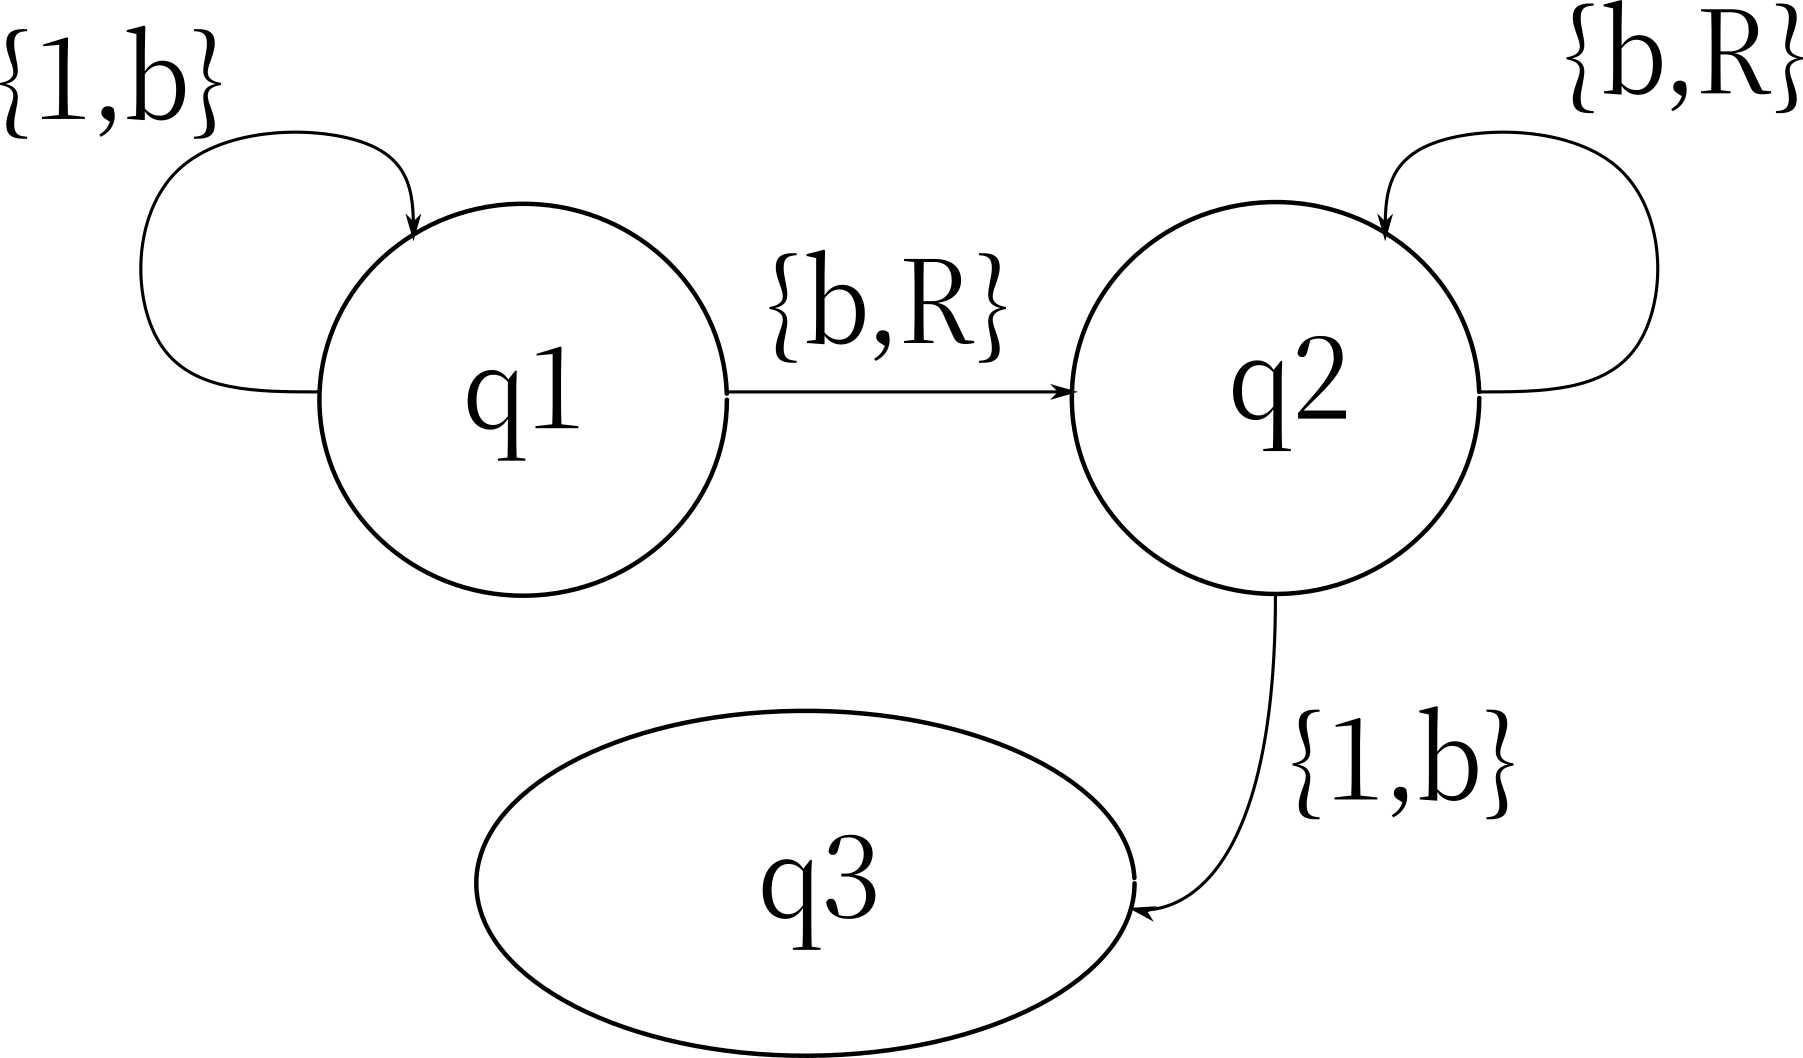
\includegraphics[ width=0.6\linewidth, height=\textheight, keepaspectratio]{./pics/mdtSomma.png}
    \caption{Grafo della macchina di Turing per le somme.}
    \label{fig:mdtSomma}
\end{figure}




\section{Altre versioni della macchina di Turing}

\subsection{Estensioni e menomazioni}

Una macchina di Turing può essere apparentemente potenziata mediante
l'estensione di essa tramite l'uso di \emph{nastri multitraccia}. In altre
parole, anziché adoperare un singolo nastro, si adoperano più nastri
contemporaneamente. La macchina di Turing viene espansa tramite l'aggiunta di
uno \emph{stato della memoria suppletiva}, che ci indica il numero del nastro
dove la macchina di Turing sta agendo. Dunque, ci possiamo immaginare una
macchina di Turing con tanti nastri e tante testine che lavorano
contemporaneamente, come illustrato in
Figura~\ref{fig:macchina-turing-multinastro}.

\begin{figure}[b]
    \centering
    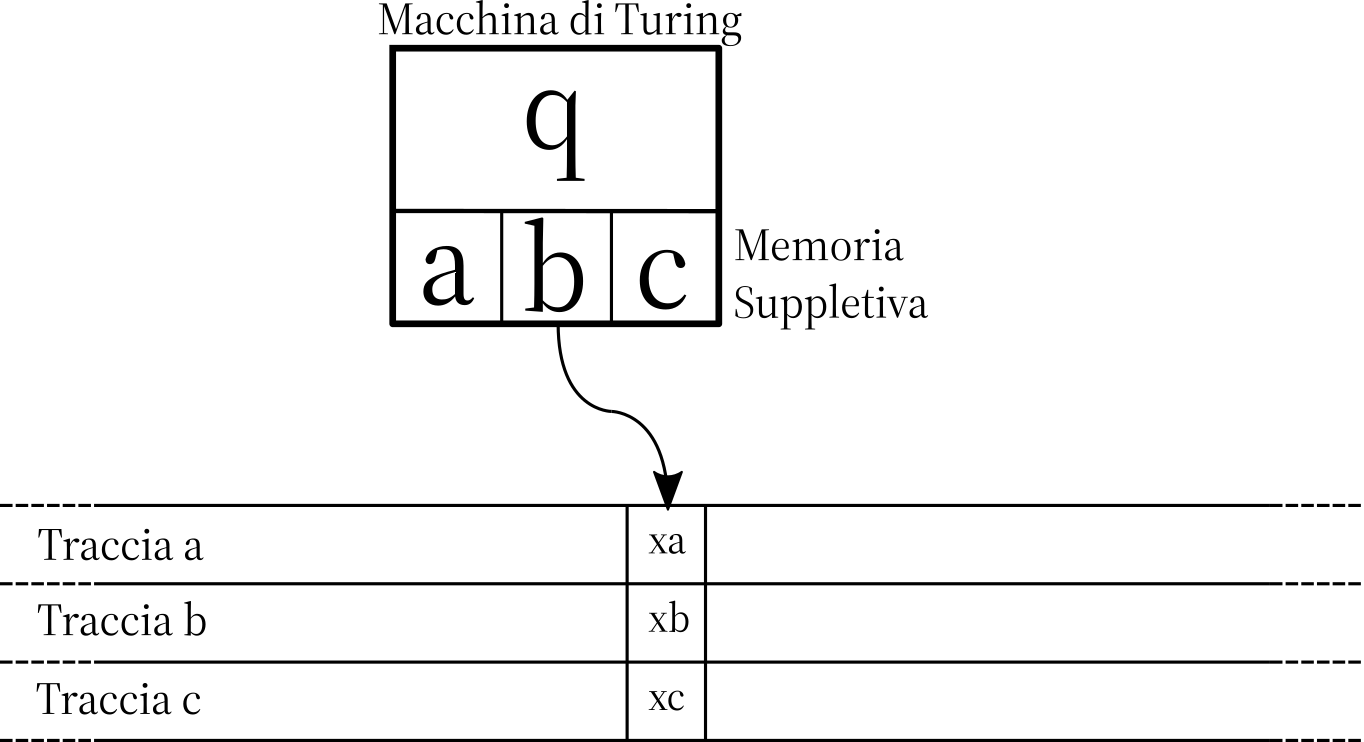
\includegraphics[ width=.8\linewidth, height=\textheight, keepaspectratio]{./pics/macchina-turing-multinastro.png}
    \caption{Macchina di Turing avente memoria con nastro multitraccia. La
    testina può collocarsi, una alla volta, su ciascuna delle nastre. La
memoria suppletiva rende possibile tenere traccia di quale nastro si sta
adoperando per l'esecuzione delle operazioni.}
    \label{fig:macchina-turing-multinastro}
\end{figure}

La domanda ora è se l'introduzione della multitraccia consenta di generare una
nuova macchina, con capacità di calcolo superiori a quelle della macchina di
Turing. La risposta è negativa: dal punto di vista della capacità computazione,
una macchina di Turing multinastro non aumenta né diminuisce le capacità. Una
macchina di Turing multinastro può essere implementata con un \emph{sistema
multitraccia} \-- in altre parole, vengono adoperate \emph{tante testine quante
sono i nastri}. Ci si può facilmente ricondurre alla macchina di Turing
convenzionale semplicemente eliminando il sistema multitraccia e facendo agire
la macchina su un nastro alla volta, o per meglio dire, una macchina di Turing
multitraccia può essere \emph{simulata} da una macchina di Turing
convenzionale: essa dunque, non produce alcun tipo di miglioramento dal punto
di vista della computazione, cioè le due macchine hanno \textbf{la stessa}
potenza computazionale (Figura~\ref{fig:mdt-equivalenza-multitraccia}). 

Tale rappresentazione, tuttavia, può avere il vantaggio di presentare una
maggiore somiglianza con il tipo di computazione svolto all'interno di un
computer moderno. Si pensi infatti alla memoria RAM, alla memoria cache, al
disco rigido e così via; una macchina di Turing può dunque ``simulare''
qualsiasi computer moderno\footnote{Un computer può a sua volta simulare da una
macchina di Turing, dal momento che possono essere applicati potenzialmente
infiniti banchi di memoria al computer \-- nella pratica, tuttavia, sappiamo
che ciò non è possibile, e i banchi di memoria non saranno mai del tutto
\emph{illmitati}.} semplicemente introducendo tanti nastri e tante tracce quante
sono quelle dei dispositivi fisici adoperati dal calcolatore moderno. Nella
fattispecie, si avrà un nastro ed una traccia per la memoria RAM, un altro
nastro ed un'altra traccia per la memoria a disco rigido, e così via. In
realtà, si tratta esclusivamente di un artificio che ci consente di tracciare
un collegamento fra il calcolatore moderno e la macchina di Turing, poiché una
macchina multinastro, sia essa multitraccia, può essere \emph{emulata} da una
macchina di Turing a nastro singolo.

Il medesimo discorso si applica anche al tentativo di \emph{menomare} la
macchina di Turing, nel senso che potremmo pensare di rendere il nastro
semi-infinito, cioè illimitato solo a destra o solo a sinistra. In tal caso,
benché questa apparente limitazione venga messa in atto, la macchina
di Turing menomata avrà di fatto la medesima capacità computazionale di quella
``standard'', perché possiamo sempre avere a disposizione una quantità
illimitata di memoria da un lato (un po' come per il modello RAM), o far uso di
trucchi come quello dell'alfabeto ausiliario $\mathcal V$ che comunque
faciliterebbero le computazioni in una situazione simile. Comunque la si veda,
una macchina di Turing non si può né potenziare né depotenziare, a meno di non
effettuare operazioni che sconvolgano il suo funzionamento, oppure
rimuovendo l'ipotesi della memoria illimitata da entrambi i lati.
\begin{figure}[b]
    \centering
    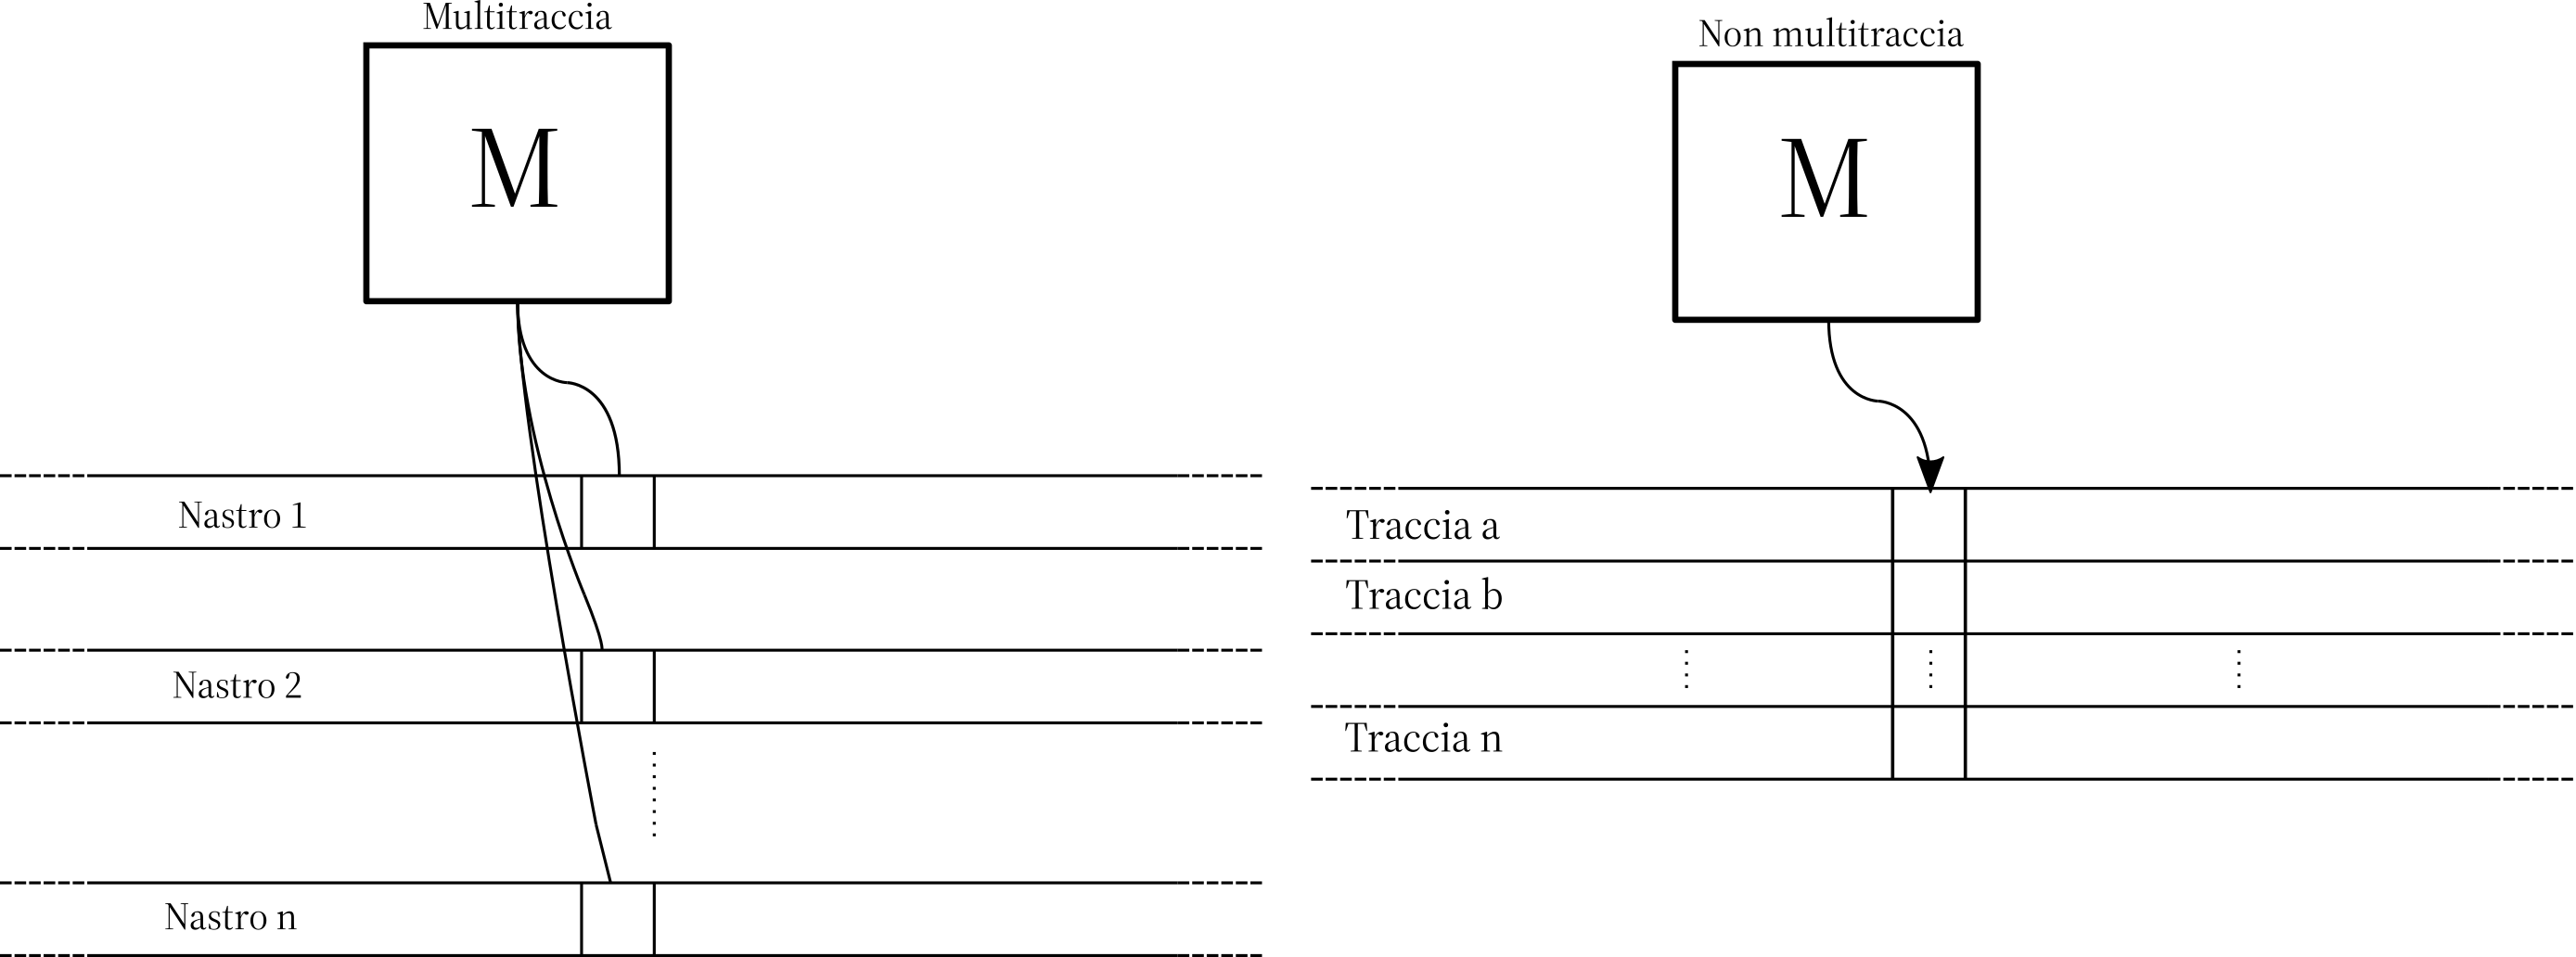
\includegraphics[ width=1.2\linewidth, height=\textheight, keepaspectratio]{./pics/mdt-equivalenza-multitraccia.png}
    \caption{Equivalenza fra una macchina di Turing a multitraccia e una
    macchina di Turing a singola testina. Non importa il numero di testine: la
macchina a singola testina potrà sempre percorrere un nastro dopo l'altro,
simulando la macchina multitraccia.}
    \label{fig:mdt-equivalenza-multitraccia}
\end{figure}

\clearpage


\subsection{Macchina RAM per \emph{accettare} stringhe}

Uno dei possibili utilizzi per una macchina di Turing (o più in generale, per
una macchina Turing-equivalente) è quello di \emph{accettore} di stringhe: la
macchina riceve in ingresso un simbolo, una \emph{stringa}; essa si dirà
\emph{accettata} qualora la computazione risultante terminasse nello stato di
\textsc{Accettazione}, altrimenti si dirà \emph{rifiutata} qualora la
computazione terminasse invece in uno stato di \textsc{Rifiuto}. Si osservi
che, in ogni caso, una macchina di Turing potrebbe ciclare all'infinito; in
quel caso saremmo di fronte ad una divergenza.

Nel modello RAM, per accettare una stringa è necessario operare una codifica.
In particolare, la stringa viene codificata in un numero naturale e la macchina
risponde con ``1'' o ``0'' a seconda che la stringa venga o meno accettata. Con
la macchina di Turing, invece, si può far intervenire direttamente uno
\emph{stato di accettazione} \textsc{Accettazione} $q_Y$ o uno \emph{stato di
rifiuto} \textsc{Rifiuto} $q_N$. La computazione terminerà qualora uno fra
questi due stati venisse raggiunto dalla macchina \-- con conseguente
accettazione o rifiuto della stringa a seconda dello stato finale. Un'altra
possibilità è quella di accontentarci di \emph{semi-decidere} riguardo
l'accettazione di una stringa, cioè di dotarsi di una macchina in grado di
riconoscere sì la stringa in questione, ma di \emph{non poterla rifiutare},
poiché in tal caso vi sarebbe un'infinita computazione, una divergenza. 

Lo stato iniziale viene di solito denotato con $q_0$, e potrebbero esserci degli
stati ulteriori ``intermedi'' fra quello iniziale e quelli terminanti. Un
esempio di accettazione è dato dalla macchina illustrata in
Figura~\ref{fig:mdtAccettazione1}. La macchina riconosce il linguaggio dato
dalle stringhe con due ``zeri'' nelle ultime due posizioni a destra, in
particolare essa riconosce tutte le stringhe che terminano con ``00''.

\begin{figure}[b]
    \centering
    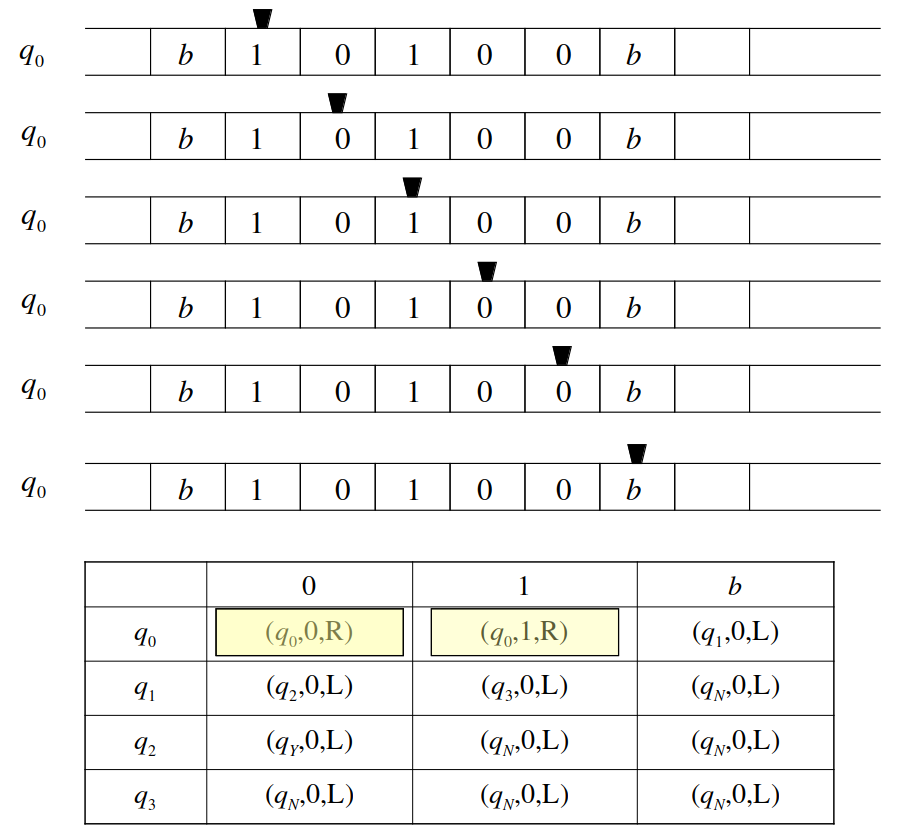
\includegraphics[ width=1.0\linewidth, height=\textheight, keepaspectratio]{./pics/mdtAccettazione1.png}
    \caption{Macchina che riconosce il linguaggio dato dalle stringhe con due $0$
nelle ultime due posizioni a destra, e suo funzionamento.}
    \label{fig:mdtAccettazione1}
\end{figure}

\clearpage

\subsection{Macchina di Turing definita a grafo}

Una macchina di Turing può anche essere ``definita a grafo''. In questo modello
di definizione, la macchina di Turing,
\begin{itemize}
    \item ha un \emph{nastro semi-illimitato} a destra, diviso in celle;
    \item ha un alfabeto \emph{ausiliario} $\mathcal V$;
    \item ha un simbolo di spaziatura $\Delta$, equivalente al simbolo
        \emph{blank} $b$;
    \item un puntatore, del tutto equivalente alla testina;
    \item un \emph{programma}, definito come \textbf{grafo finito orientato},
        con i vertici definiti come \emph{stato}. Vi è uno stato di inizio,
        indicato con \textsc{Inizio}, e un sottoinsieme eventualmente vuoto di
        stati di arresto, indicati con \textsc{Accettazione}. I nodi del grafo
        sono collegati da \emph{archi}.
\end{itemize}

Ciascun arco è della forma
\begin{figure}[h]
    \centering
    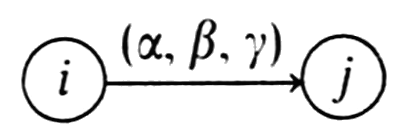
\includegraphics[ width=.4\linewidth, height=\textheight, keepaspectratio]{./pics/mdtGrafo.png}
    \label{fig:mdtGrago}
\end{figure}


dove $$\alpha \in \Sigma \cup \mathcal V \cup \{\Delta\}, \beta \in \Sigma \cup
\mathcal V \cup \{\Delta\} \mbox{ e } \gamma \in \{L, R\}.$$ Dunque, siamo
nello stato $i$; la macchina legge $\alpha$, scrive $\beta$ al posto di
$\alpha$, e infine va a destra oppure a sinistra a seconda che il simbolo
$\gamma$ sia pari ad $R$ o ad $L$. Una proprietà importante è che tutti gli
archi che partono da un medesimo vertice devono avere $\alpha$ diversi.

\begin{figure}[h]
    \centering
    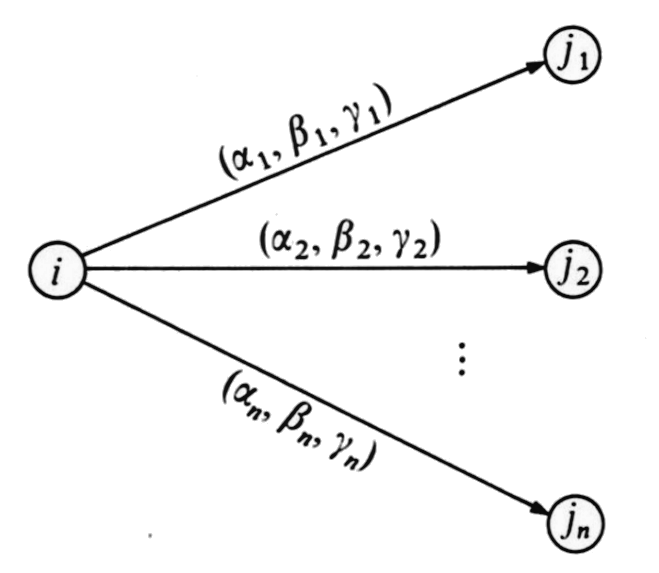
\includegraphics[ width=.4\linewidth, height=\textheight, keepaspectratio]{./pics/mdtArchiDiversi.png}
    \label{fig:mdtArchiDiversi}
\end{figure}

Se così non fosse, si avrebbero più cammini possibili per uno stesso
simbolo~\--~un'ipotesi che come vedremo in seguito sarà violata assumendo che
una macchina di Turing possa non essere di tipo \emph{deterministico}.

\begin{figure}[b]
    \centering
    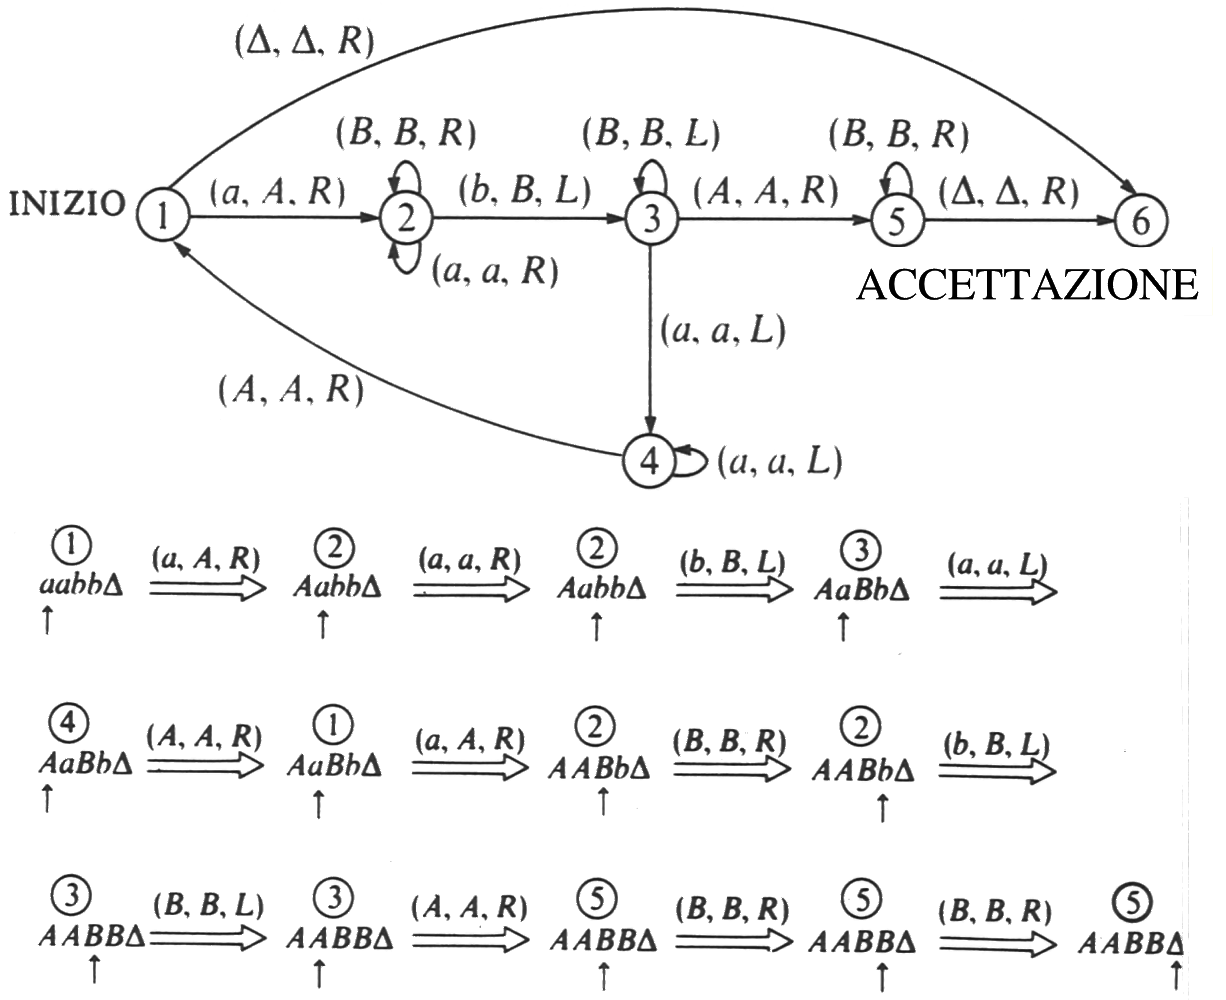
\includegraphics[ width=1.0\linewidth, height=\textheight, keepaspectratio]{./pics/mdtLetturaStringaSpeciale.png}
    \caption{Macchina di Turing in grado di riconoscere una stringa della forma
    $a^nb^n | n\geq 0$.}
    \label{fig:mdtLetturaStringaSpeciale}
\end{figure}

Si possono disegnare le macchine di Turing direttamente con i grafi. Il
problema espresso in Figura~\ref{fig:mdtLetturaStringaSpeciale} è il problema
del riconoscimento di una stringa avente forma $a^nb^n | n\geq 0$, ed è molto
noto nella teoria della computabilità, poiché è un tipico esempio di problema
che è risolubile da una macchina di Turing, ma \textbf{non risolubile} mediante
una \emph{macchina a stati finiti}. Tali macchine, infatti, non presentano
alcun tipo di \emph{memoria}, e dunque per questa particolare mancanza non sono
in grado di risolvere il problema del riconoscimento. La macchina di Turing,
invece, è in grado di risolverlo in virtù della sua superiore potenza di
computazione.

Un ulteriore esempio dell'applicazione della macchina di Turing a grafo è
mostrato in Figura~\ref{fig:mdtConcatenazioneStringhe}, dove la macchina in
questione è in grado di concatenare due stringhe a due lettere $a$ e $b$.

\begin{figure}[b]
    \centering
    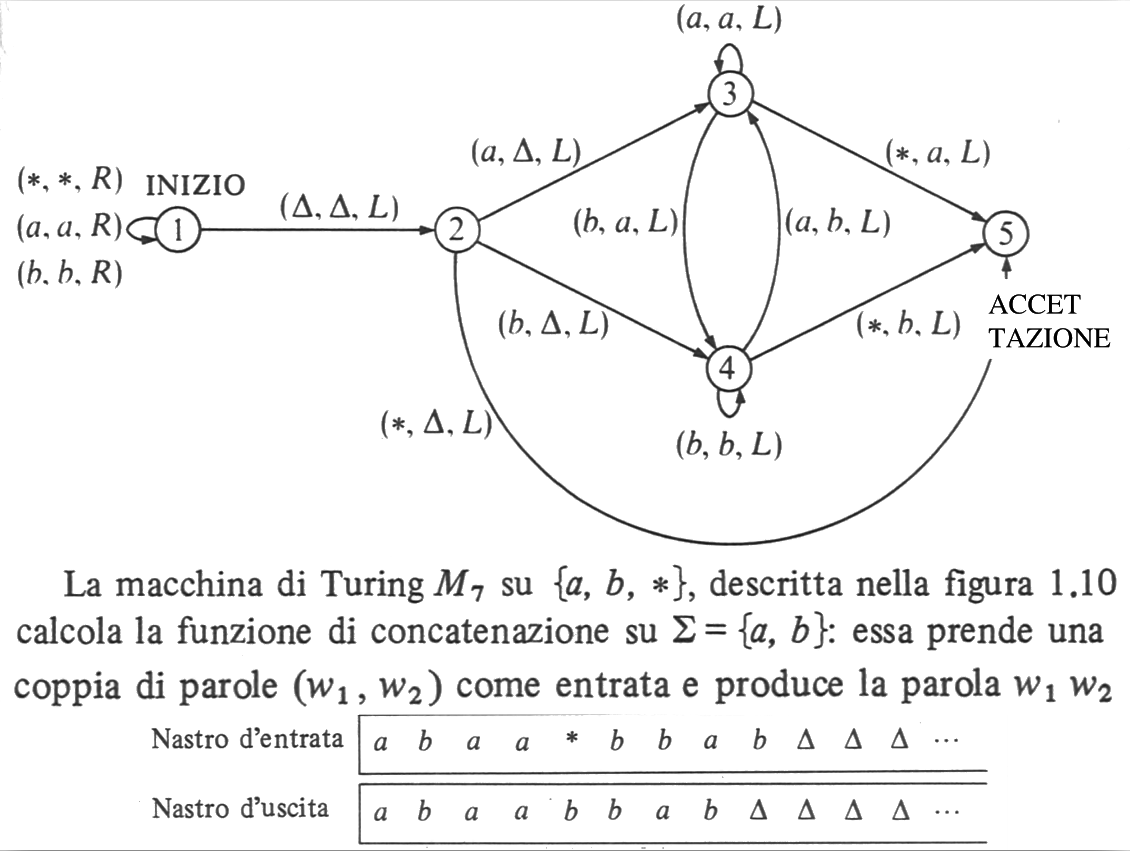
\includegraphics[ width=1.0\linewidth, height=\textheight, keepaspectratio]{./pics/mdtConcatenazioneStringhe.png}
    \caption{Macchina di Turing in grado di concatenare due stringhe $w_1$ e $w_2$.}
    \label{fig:mdtConcatenazioneStringhe}
\end{figure}



\chapter{Le macchine non deterministiche}

\section{Gerarchie delle potenze di calcolo}

Oltre alla macchina di Turing nelle sue varie versioni, sono possibili altre
tipologie di macchine, con vari livelli di gerarchia fra potenze di calcolo. Il
seguente elenco ne illustra alcune,

\begin{itemize}
    \item macchine a \emph{stati finiti}: in questo caso, hanno $0$
        \emph{memorie push-down} \-- le macchine a stati finiti sono le meno
        potenti in assoluto dal punto di vista computazionale, e non sono in
        grado di risolvere il problema del riconoscimento di stringhe $a^n
        b^n$, espresso in Figura~\ref{fig:mdtLetturaStringaSpeciale};
    \item macchine a \emph{$1$ memoria push-down}: dotate di una memoria
        push-down che implementa una pila FIFO (\emph{first in\----first out}),
        hanno una maggiore potenza di calcolo rispetto alla macchina a stati
        finiti;
    \item macchine a \emph{$2$ memorie push-down}: dotate di $2$ memorie
        push-down, esse sono equivalenti alla macchina di Turing.
    \item macchine \emph{di Post}: sono uno speciale tipo di macchine a memorie
        push-down, aventi una memoria di tipo LIFO (\emph{last in\----first
        out}). Esse sono equivalenti alle macchine a $2$ memorie push-down e
        alle macchine di Turing;
    \item una macchina con $3$ o più pile push-down non fornisce vantaggi dal
        livello della potenza computazionale, e sono tutte Turing-equivalenti
        \-- il vantaggio è semmai nella semplificazione di calcoli fornita
        dall'introduzione della pila aggiuntiva.
\end{itemize}


Perciò, la gerarchia delle potenze di calcolo è la seguente, dall'alto verso il basso:
\begin{enumerate}
    \item Macchine non deterministiche di Turing, con due memorie
        push-down~\----~Macchine di Turing, Modello RAM, Macchine di Post,
        macchine finite con due memorie push-down (sono in grado di accettare
        $\{a^n b^n a^n| n \geq 0\}$). Si potrebbe dimostrare che le macchine di
        Turing deterministiche e non deterministiche hanno la medesima potenza
        di calcolo; 
    \item Macchine finite non deterministiche con una memoria push-down, sono
        in grado di riconoscere $\{w w^R | w\in\{a,b\}^*\}$\footnote{Il
        \emph{nodo di decisione} che introduce il non determinismo serve per
    gestire la situazione data dall'incapacità di riconoscere il punto di
rottura $ww^R$, cioè il punto in cui finisce $w$ ed inizia $w^R$. Con il non
determinismo, ogniqualvolta si arriva al nodo di decisione si tengono valide
entrambe le possibilità \-- dunque, è più potente della macchina ad una memoria
push-down, ma deterministica.};
    \item macchine finite con una memoria push-down, riconoscono $\{a^n
        b^n|n\geq 0\}$;
    \item Macchine finite non deterministiche senza memorie push-down \----
        macchine finite senza memorie push-down \---- automi finiti.
\end{enumerate}


\subsection{Alcune definizioni sulle stringhe}

Sia dato l'alfabeto $\Sigma^*$. Faremo uso di tre fondamentali funzioni
definite su $\Sigma^*$:
\begin{itemize}
    \item l'operazione $testa(x)$, che fornisce la ``testa'' di una stringa,
        ovverosia la lettera di estrema sinistra della parola $x$;
    \item l'operazione $coda(x)$, la quale invece fornisce la ``coda'' di una
        stringa, o la stringa privata della sua testa $x$;
    \item l'operazione $\sigma \cdot x$, che \emph{concatena} la lettera
        $\sigma$ e la parola $x$, per formare un'unica parola nuova.
\end{itemize}


\section{La macchina di Turing non deterministica}

La macchina di Turing effettiva è di tipo \emph{deterministico}. Nella
fattispecie, una macchina deterministica definita a grafo vede ciascun arco che
parte dallo stesso vertice avere \emph{simboli diversi}. Se ciò non fosse vero,
leggendo un unico simbolo $\alpha_i$ e trovandosi nello stato $q_j$ la macchina
di Turing non potrebbe ``scegliere'' il percorso, poiché ne esisterebbe più di
uno. Viceversa, una macchina \emph{non deterministica} rompe questa assunzione,
e permette alla macchina di compiere una scelta, sia essa arbitraria o del
tutto casuale, riguardo quale percorso seguire fra i vari disponibili. 

Il \emph{non determinismo} viene introdotto per due ragioni:
\begin{itemize}
    \item si desidera osservare se una macchina di Turing non deterministica
        sia o meno più \emph{potente} di una macchina di Turing deterministica;
    \item si cerca di valutare se possano esistere differenti paradigmi di
        computazione (ad esempio, computazione parallela).
\end{itemize}

Una \emph{macchina di Turing non deterministica} può avere nel suo diagramma di
flusso dei \emph{nodi di decisione} dove a fronte di un medesimo simbolo vi
sono \emph{più archi possibili} \-- il non determinismo viene dunque introdotto
da questo fenomeno: una macchina di Turing non deterministica può scegliere il
suo percorso con una legge non deterministica, ma semmai dettata dal caso o da
una \emph{scelta arbitraria}. 

Una macchina non deterministica accetta l'idea che vi siano più possibilità di
sviluppo di una computazione a fronte di un medesimo simbolo identificato sul
nastro e associato ad un determinato stato; sono dunque possibili diversi
percorsi di computazione. Questo tipo di macchina, ad esempio, potrebbe
percorrere \emph{tutti i percorsi simultaneamente}, concependo il
\textbf{parallelismo} nella computazione, nel senso che più possibilità e
percorsi nel calcolo sono possibili. Questa potenzialità, apparentemente di
gran lunga migliorativa, \textbf{non aumenta} la potenza di calcolo della
macchina di Turing. Una macchina di Turing deterministica può, infatti,
simulare una macchina non deterministica: è sufficiente compiere una ricerca
per ogni diramazione dell'albero dei nodi, con un aumento
esponenziale\footnote{L'aumento esponenziale è dovuto al fatto che, ad ogni
diramazione effettuata da una macchina di Turing non deterministica, la
relativa macchina deterministica dovrà (almeno) sdoppiarsi su $2$ percorsi.}
del numero di operazioni da effettuare, ma pur sempre un'operazione
realizzabile e computabile da una macchina di Turing. Una macchina non
deterministica ha dunque il potenziale vantaggio di poter risolvere problemi in
\emph{tempo lineare} che dalla macchinia deterministica sarebbero risolti in in
tempo esponenziale.

In questo caso, il parallelismo è insito nella macchina non deterministica;
supponendo di voler risolvere un problema di accettazione, la stringa si
considera \emph{accettata} qualora uno qualunque fra i percorsi possibili
incappa nello stato di \textsc{Accettazione}. Una parola $w \in \Sigma^*$ si
dice \emph{accettata} da una macchina di Turing non deterministica se esiste
una computazione della macchina $M$ che cominci con entrata $x=w$, e che
termini ad un arresto con lo stato di \textsc{Accettazione}. Se $w$ non viene
accettata e lo stato di arresto è quello del \textsc{Rifiuto}, allora si dice
che $w$ è \emph{rifiutata}. In alternativa, siamo di fronte ad un ciclo
infinito $w \in ciclo(M)$, cioè dinanzi ad una divergenza.

Possiamo quindi pensare ad una macchina di Turing non deterministica
come ad un macchina avente per ogni cella, nella matrice di transizione, un
\emph{insieme} $\delta(q,s)$ di triple $q_i, s_i, \alpha_i$, dove $\alpha_i \in
\{L,R\}$ e ad ogni elemento dell'insieme corrisponde una possibile scelta da
compiere arbitrariamente o casualmente; dunque da lì è ottenuto il non
determinismo della macchina. Ogni possibile scelta genererà un diverso ramo
nell'albero della computazione \-- per l'accettazione di un simbolo è
sufficiente che uno \emph{qualsiasi} fra i rami di computazione termini nello
stato di \textsc{Accettazione}. Dunque, benché una macchina di Turing non
deterministica non \textbf{aumenti} la potenza di calcolo intrinseca della
macchina, essa consente la \textbf{parallelizzazione} dei possibili percorsi
della computazione, rendendo di fatto possibile risolvere in tempo lineare
problemi che sarebbero risolubili (comunque), ma in tempo esponenziale per una
macchina deterministica.

\subsection{Equivalenza fra macchine non deterministiche e macchine multinastro}

\begin{thm}
    Ogni macchina di Turing non deterministica ha un equivalente macchina di
    Turing deterministica multinastro.
\end{thm}

\textsc{Dimostrazione} \---- Una traccia della dimostrazione è una ricerca
nell'albero di computazione. Con almeno due nastri, si simula con uno la
macchina non deterministica mentre con l'altro si collezionano tutti i
possibili $k$ ``prossimi passi'' della tabella di transizione. La macchina di
Turing deterministica allora controllerà tutte le configurazioni
stato\----simbolo, livello per livello, dell'albero di computazione. Lo stato
finale di \textsc{Accettazione} terminerà la computazione complessiva.

L'idea è quella, dunque, di \emph{simulare} il non determinismo compiendo un
numero crescente in modo esponenziale di passi, uno per ogni ramo dell'albero
non deterministico di computazione.

\begin{thm}
    Ogni macchina di Turing non deterministica $T_M(n)$ ha un equivalente
    macchina di Turing deterministica con ordine $2^{O(T_M(n))}$.
\end{thm}

\textsc{Dimostrazione} \---- Una traccia può essere che il numero massimo di
foglie è $O(b^{T_M(n)})$, dove $b$ è il numero di figli. Il tempo per viaggiare
dalla radice lungo ogni ramo è, per una macchina multinastro,
$$O(T_M(n)b^{T_M(n)}) = 2^{O(T_M(n))},$$ mentre per una macchina a nastro
singolo $$(2^{O(T_M(n))})^2 = 2^{O(2T_M(n))} = 2^{O(T_M(n))},$$ dunque l'ordine
è lo stesso.


\begin{figure}[h]
    \centering
    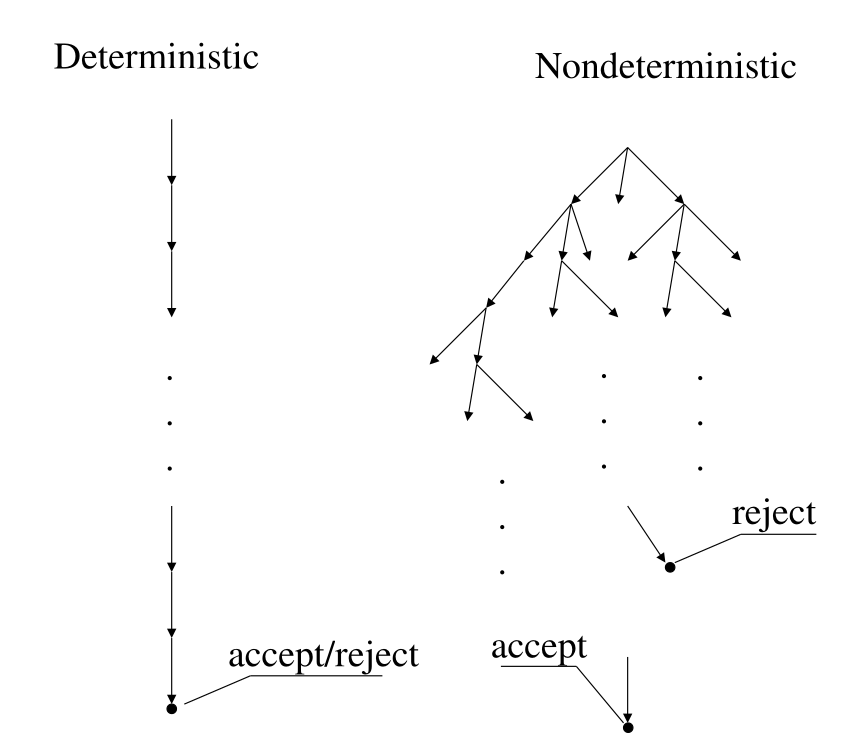
\includegraphics[ width=1.0\linewidth, height=\textheight, keepaspectratio]{./pics/ndtmEsempio.png}
    \caption{Esempio di computazione ``in parallelo'' effettuata dalla macchina
    non deterministica (a destra), e simulazione da parte della macchina
deterministica (a sinistra).}
    \label{fig:ndtmEsempio}
\end{figure}

In altre parole, una macchina non deterministica è in grado di ``evocare'' un
numero esponenziale ed arbitrariamente elevato di macchine di Turing
deterministiche \-- tale funzionalità però è irrealizzabile, poiché
corrisponderebbe a dotare la propria macchina di un numero arbitrario di unità
di calcolo, ciascuna per ogni possibile passo della computazione, per farle
lavorare in parallelo. Se ciò fosse invece possibile nel mondo materiale,
potremmo effettivamente risolvere problemi difficilmente trattabili in tempo
polinomiale, rendendoli di fatto trattabili.



\chapter{Le reti neuronali di Hopfield}

Le \emph{reti neuronali} incarnano un diverso paradigma di computazione
rispetto a quello della computazione procedurale algoritmica. Storicamente esse
prendono spunto dalla natura, in particolare dal concetto di \emph{neurone},
inteso come singola unità di calcolo, dotata di input, di output e di una
\emph{funzione caratteristica}. Diversamente dall'idea della computazione
procedurale, dove la \emph{complessità} è definita tramite la complessità di
tipo computazionale (o temporale), le reti neuronali esprimono la loro
complessità attraverso la \textbf{complessità strutturale}, o
\textbf{complessità circuitale}. In altre parole, per risolvere un problema
l'idea è quella di aumentare la complessità di tipo circuitale della rete, ad
esempio aggiungendo neuroni, facendo variare le conduttanze, adoperando diverse
funzioni di attivazione. La computazione è di tipo \emph{collettivo}, ed emerge
come proprietà dell'\emph{evoluzione dinamica} della rete. Ogni decisore
locale, detto \emph{neurone}, non ha visibilità della computazione globale, e
svolge il proprio compito localmente \---- ogni decisore locale concorre alla
soluzione globale in modo sfumato, con il proprio valore in stato alto o basso:
la rete è \textbf{robusta} rispetto a malfunzionamenti locali, poiché ciascun
neurone singolo non è critico e non può pregiudicare l'intera rete da solo.
Spesso è addirittura possibile eliminare qualche neurone senza che la rete ne
risenta in maniera rilevante.

Dal punto di vista strettamente logico, il paradigma di computazione a reti
neuronali è l'unico paradigma radicalmente differente da quello procedurale,
mentre il paradigma \emph{a DNA}\footnote{TEST FIXME TODO Trattasi di un paradigma di calcolo
dove si va a cercare lo spazio delle soluzioni, e si eleggono quelle più
``performanti'' \---- talune soluzioni saranno la base dalla quale saranno
definite le successive soluzioni, convergendo dunque alla soluzione. La potenza
di questo metodo è quello di potersi permettere una ricerca esauriente della
soluzione, poiché ciascun DNA è infinitesimamente piccolo, e dunque può essere
esaminato in parallelo.} è una tipologia di calcolo che, nella realtà, non
differisce sostanzialmente dal metodo procedurale.

Esistono due filoni di reti neuronali; il primo associato ai
\textbf{perceptron}, macchine a strati che fungono da riconoscitori di pattern
e configurazioni. Le variabili di ingresso rappresentano un ente, una
configurazione del sistema esterno, e il perceptron è in grado di fornire in
output una risposta che consente di riconoscere tale configurazione o pattern
in base a come essa sia stata configurata e ai suoi parametri. I
cosiddetti \emph{multilayer perceptron} sono particolari casi di perceptron,
aventi i neuroni organizzati in \emph{layer}. Vi sono due layer ``principali''
di input e di output, e dei layer ``nascosti'' (in gergo \emph{hidden layer})
dove avvengono ulteriori passaggi intermedi. Tipicamente, i layer sono
costituiti da neuroni aventi particolari \emph{funzioni di attivazione}. Le
funzioni di attivazione sono ciò che determina il comportamento dei singoli
neuroni \-- in particolare, esse determinano la maniera in cui un neurone debba
attivarsi o rimanere nello stato di quiete. I perceptron hanno la
caratteristica fondamentale di essere \emph{feed-forward}, cioè di avere una
\emph{direzionalità} nella rete: i neuroni non possono essere connessi in
cicli, cioè il corrispondente grafo è aciclico. L'infrastruttura dei perceptron
ha un comportamento di tipo euristico, cioè non esiste alcun modello di
computazione associato alla struttura, non vi sono teoremi e, di fatto, manca
un apparato matematico. Per modellare un perceptron, solitamente, si adottano
tecniche euristiche di \emph{machine learning}, con apprendimenti automatici.

Il secondo filone, invece, è quello della \emph{rete di Hopfield}; tale filone
sarebbe in grado, in linea di principio, di \textbf{risolvere problemi} di
natura matematica. Mediante una rete di Hopfield è possibile risolvere ad
esempio il \emph{travelling salesman problem}, un problema presumibilmente
intrattabile\footnote{``Presumibilmente'' si riferisce al fatto che, fino ad
ora, nessuno è riuscito a dimostrare né che tale problema può essere risolto in
tempo polinomiale, né che non può esserlo.}. Le reti di Hopfield, diversamente
dai perceptron, possono essere modellate con grafi ciclici, dunque esistono
percorsi ciclici fra neuroni.

Ambedue i modelli, tuttavia, non possono essere considerati dei veri e propri
modelli alternativi a quello della macchina di Turing, in primis per l'assenza
dell'apparato matematico, e in secondo luogo poiché è stato dimostrato che
nella sostanza e sotto opportune ipotesi una rete neurale ha la stessa potenza
di calcolo del modello RAM. Le reti neurali quindi, non sono un modello di
computazione alternativo, semmai sono un \emph{paradigma} differente.

Le reti neuronali hanno avuto grande successo in $3$ periodi storici:
\begin{itemize}
    \item all'inizio degli anni $40$ \-- nel $1948$ fu fornito il primo modello
        di neurone e rete neuronale. L'idea fu quella di avvalersi di una
        macchina fisica per simulare il comportamento dei neuroni naturali,
        presenti nel nostro cervello
        (Figura~\ref{fig:retiHopfieldNeuroneParagone}. All'epoca uscirono anche
        articoli su memorie a breve e lungo termine adoperando reti neuronali;
    \item durante gli anni $80$ \-- nei primi anni $80$, Hopfield individuò un
        modello di reti neuronali che associava le reti neuronali ad un
        particolare modello matematico; qualità che prima era assente. Si
        tratta di una caratteristica fondamentale: quando si cerca di risolvere
        problemi con le reti neuronali, l'assenza di teoremi (ad esempio,
        quelli asintotici) non ci permette di stabilire la \emph{qualità} di
        una soluzione, oppure se la computazione andrà in qualche maniera a
        buon fine. Dunque, l'assenza di un buon apparato matematico che faccia
        da base alle reti neuronali è il principale svantaggio di tale
        paradigma. Hopfield riuscì a fornire la soluzione di alcuni fra questi
        problemi matematici, suggerendo la possibilità di risolvere problemi,
        come ad esempio quello sopra citato del \emph{travelling salesman
        problem}. Ci fu allora una corsa dal punto di vista scientifico
        riguardo la possibilità di risolvere in maniera efficiente i problemi
        presumibilmente intrattabili. Si può dimostrare, tuttavia, che la
        potenza di computazione di una macchina di Hopfield \textbf{non è
        superiore} alla capacità di computazione della macchina di Turing. Con
        una macchina di Hopfield non è dunque possibile risolvere in tempo
        polinomiale problemi che non sono risolubili in tale maniera già dalla
        macchina di Turing \-- vi è dunque l'\emph{equivalenza} fra le due
        macchine. Le reti di Hopfield caddero pertanto ben presto in disuso;
    \item il terzo ed ultimo periodo d'oro delle reti neuronali è il giorno
        d'oggi, dove la potenza di calcolo superiore delle macchine moderne
        apre la strada ad un ampio uso delle reti neuronali in applicazioni
        concrete, che si avvalgono della pura potenza computazionale di gran
        lunga maggiore rispetto al passato per produrre risultati in tempo
        apprezzabile.
\end{itemize}

\begin{figure}[h]
    \centering
    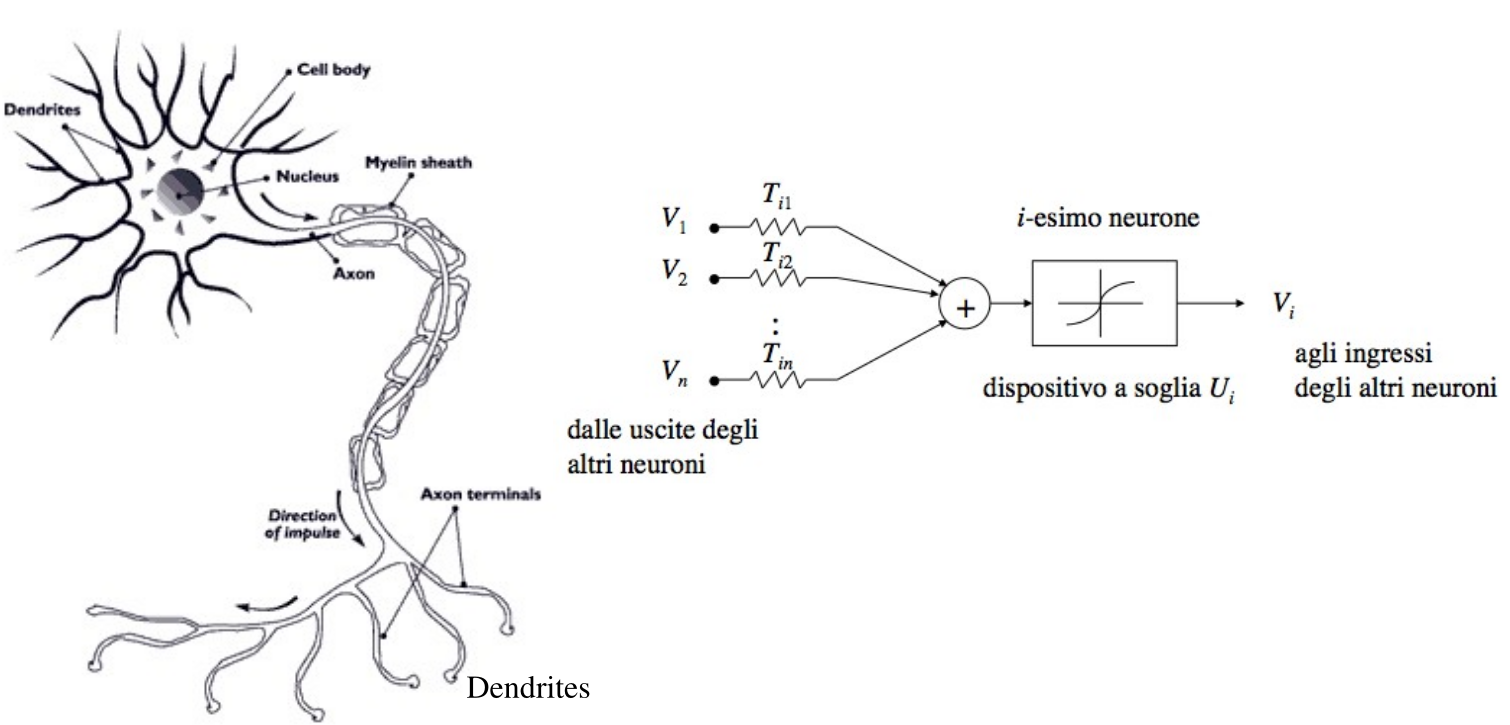
\includegraphics[ width=1.0\linewidth, height=\textheight, keepaspectratio]{./pics/retiHopfieldNeuroneParagone.png}
    \caption{Paragone fra neurone naturale e neurone di Hopfield. Si osservino
    innanzitutto le somiglianze fra le due strutture. La somiglianza principale
è il fatto che anche i neuroni naturali presentano vari input e vari output,
collegati con diversi altri neuroni. Tipicamente, anche un neurone naturale
presenta una vera e propria funzione di attivazione, che ne determina il
comportamento ``a soglia''. La stimolazione del neurone naturale è stimolata da
segnali continui, sebbene il \emph{firing} (eccitazione del neurone) avvenga in
maniera discreta.}
    \label{fig:retiHopfieldNeuroneParagone}
\end{figure}



\section{Il neurone reale ed il neurone simulato}

Una macchina di Hopfield simula un neurone reale. Vi sono all'incirca $10^{11}$
neuroni (cento miliardi) nel cervello, i quali formano una rete neuronale di
una complessità strabiliante. Il cervello è in grado di svolgere una quantità di
compiti enorme, in modo molto efficiente \-- il cervello è infatti la struttura più
complessa che esista nell'universo noto, non paragonabile ad alcun altro tipo
di struttura, sia essa già esistente in natura o creata artificialmente. I
segnali elettrici nel cervello si sviluppano nell'ambito dei \emph{segnali
continui}, tuttavia il funzionamento di un neurone si svolge, in realtà, 
propriamente nell'ambito dei \emph{segnali discreti}. Vi sono infatti i
cosiddetti \emph{spike}: un neurone si ``eccita'' o si ``rilassa'',
manifestando dunque un comportamento discreto secondo questo punto di vista,
anche se il sottostante segnale è, di fatto, un segnale elettrochimico di
natura continua.

\section{La rete discreta di Hopfield}

La \textbf{rete discreta di Hopfield} è composta da singoli neuroni, modellati tramite
le tensioni elettriche. Ciascun $i$-esimo neurone ha la forma illustrata in
Figura~\ref{fig:retiHopfieldNeuroneParagone}: esso è dotato di $n$ ingressi
$V_j$ collegati ad altri neuroni, delle ``conduttanze'' dal valore $T_{i,j}$
che simulano i contatti fra neuroni\footnote{Il valore di tali conduttanze
\emph{varia} in funzione del tempo, in particolare in base a quanto
frequentemente il neurone viene sollecitato \-- questo modello artificiale è
basato su quello reale, dove i dendriti variano a seconda della frequenza con
cui il neurone viene sollecitato.}; ciascuno degli ingressi si sommerà e la
somma verrà valutata dalla \emph{funzione di attivazione}, collocata nella
parte centrale. Il neurone di Hopfield è un dispositivo dal comportamento
\emph{a soglia} (sigmoide): la funzione di attivazione pesa la somma degli
ingressi, producendo un output $V_{i}$ \textbf{pressoché discreto} da dirigere
agli ingressi di altri neuroni. Nel caso discreto, la soglia si dice essere
\emph{rigida}: stabilita la soglia $U_i$ del neurone, avremo due possibilità,
\begin{itemize}
    \item o $V_{i} = 1$ se $\sum_{j\neq i} T_{ij} V_j > U_i$;
    \item oppure $V_{i} = 0$ se $\sum_{j\neq i} T_{ij} V_j < U_i$;
\end{itemize}

cioè la soglia determina il comportamento che l'uscita del neurone presenta a
seconda dei valori dell'ingresso (o più precisamente, a seconda di quanto vale
la loro somma pesata dalle conduttanze $T_{ij}$).

In un certo senso quindi, si può affermare che un neurone di Hopfield si
comporta ``discretamente'', nel senso che il suo valore di uscita può assumere
valori o prossimi allo $0$, o prossimi all'$1$, con possibili valori intermedi
dipendenti esclusivamente dalla forma che la funzione di attivazione presenta
(si assume che essa difficilmente possa avere la forma di un perfetto gradino,
e che esistano porzioni di essa in cui il valore è compreso fra $0$ ed $1$ con
valori continui. Ciononostante, è sufficiente interpretare il segnale continuo
in senso discreto, cioè valutando con un'opportuna soglia il valore dell'output
di un neurone, un po' come avviene nei circuiti digitali). Nella fattispecie,
consideriamo un comportamento a soglia di tipo ideale, cioè nel quale la
funzione di attivazione è un gradino ideale.

Per quanto concerne le reti di Hopfield, è importante fare due osservazioni. La
prima è che se $V_i = 1$, in ogni caso (sia che fosse già in $1$ o che fosse in
$0$) si ha che $\Delta V_i \geq 0$. Viceversa, se $V_i = 0$, in ogni caso si
avrà che $\Delta V_i \leq 0$: questa cruciale osservazione ci permette di
stabilire che

$$\Delta E = -\Delta V_i (\sum_{j \neq i} T_{ij}V_j - U_i) \leq 0,$$ cioè la
variazione di energia, ovvero la potenza, \emph{è sempre minore di zero}. La
\textbf{variazione dell'energia della rete}, dunque, \textbf{è sempre
negativa}. Questo fatto è di fondamentale interesse, poiché ci definisce la
maniera in cui la rete tende ad evolversi, riducendo ad ogni passo la quantità
di energia totale.

La seconda importante osservazione è che nel caso in cui si assuma una
simmetria della rete (cioè quando il neurome $i$-esimo incide sul neurone
$j$-esimo tanto quanto il neurone $j$-esimo incide su quello $i$-esimo),
l'energia $E_i$ del neurone $i$-esimo sarà pari a

$$E_i = -V_i(\sum_{j\neq i} T_{ij}V_{j} - U_i),$$ e sotto ipotesi $T_{ij} =
T_{ji}$, si ha infine che l'\textbf{energia della rete di Hopfield} $E$ è pari
a

\begin{equation}
    E = -\frac{1}{2} \sum_{ij, j\neq i} T_{ij}V_i V_j + \sum_{i} V_i U_i,
\end{equation}

un termine corrispondente ad una \emph{forma quadratica}.

Dunque, per come è stata impostata la rete e per le due osservazioni effettuate
sopra, l'energia della rete decresce sempre: tenendo conto di tale risultato
fondamentale, si può costruire una rete di Hopfield.

\begin{figure}[h]
    \centering
    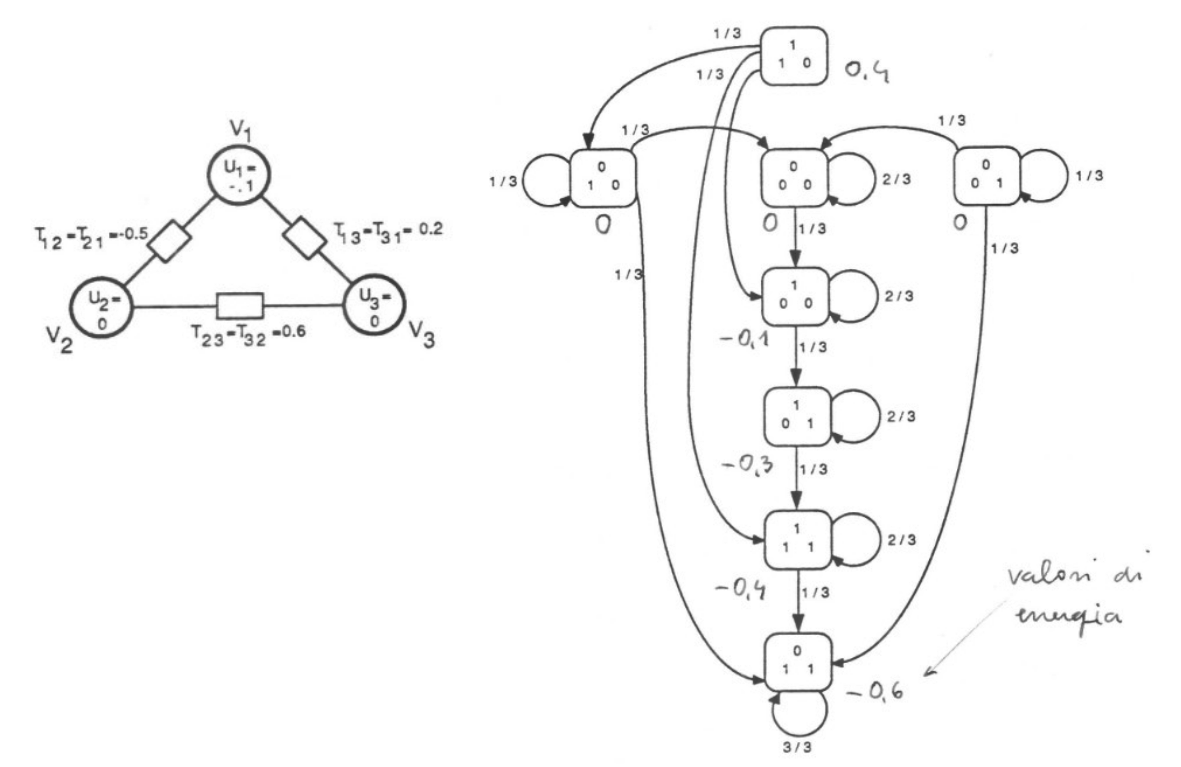
\includegraphics[ width=1.1\linewidth, height=\textheight, keepaspectratio]{./pics/reteHopfieldBase.png}
    \caption{Rete di Hopfield costituita da $3$ neuroni, collegati ad anello.
    Ciascun neurone è collegato ad ogni altro mediante una particolare
conduttanza $T_{ij}$, che soddisfa la relazione di simmetria $T_{ij} = T_{ji}$.
Si osserva, sulla destra, l'evoluzione probabilistica della rete, con
decremento dell'energia. Non sono ammessi incrementi energetici.}
    \label{fig:reteHopfieldBase}
\end{figure}

I neuroni possono, almeno secondo una particolare configurazione iniziale, non
presentare un valore dell'uscita adeguato ai valori presenti all'ingresso. In
ogni istante discreto, ciascun neurone ha la medesima probabilità di essere
eccitato (firing), cioè si può verificare la compatibilità del suo valore di
uscita sulla base della somma pesata degli ingressi. Potrebbe darsi che la
somma degli ingressi sia maggiore della soglia $U_i$, ma che il valore d'uscita
sia basso, o viceversa che la somma degli ingressi presenti un valore basso, con uscita alta \-- in tal caso, avremo che il neurone \emph{non è soddisfatto}, cioè
è in una condizione di disagio. Esso vorrebbe vedere la propria coerenza
soddisfatta: tanto più i neuroni di una rete di Hopfield sono soddisfatti,
tanto minore sarà l'energia associata allo stato che produrrà tale
soddisfacimento. 

Il modello che Hopfield suggerisce per superare tale
difficoltà è quello di \emph{verificare}, neurone per neurone, la coerenza fra i
valori ai suoi ingressi e il suo valore d'uscita, con una verifica che avviene
in tempo discreto. Qualora non ci fosse coerenza, il neurone andrà modificato,
ottenendo un nuovo stato della rete. In ogni caso, il fenomeno a cui si assiste
è quello per cui ad ogni variazione l'energia della rete cala complessivamente.
Il procedimento di verifica proposto da Hopfield è del tutto aleatorio, e consiste
nell'aggiustamento progressivo dei pesi, calando di volta in volta di energia. Secondo la legge dei grandi numeri, la rete si evolverà percorrendo i vari passi, fino a terminare in una configurazione a minima energia: la configurazione di \emph{minimo locale} dell'energia della rete.
Una volta raggiunta la configurazione di minimo locale dell'energia, non
si può più uscire dalla configurazione. Il minimo dell'energia della rete,
dunque, dovrà corrispondere in qualche maniera alla soluzione cercata. 

Risolvere un problema con una rete di Hopfield, dunque, necessita di un passo
iniziale di \emph{codifica}, cioè che il procedimento di minimazione
dell'energia della rete, cioè la minimazione di una forma quadratica, abbia un
corrispettivo con la soluzione del problema desiderato. In linea di principio,
avendo a disposizione una valida codifica, è possibile risolvere il problema
semplicemente minimizzando l'energia della rete corrispondente, con il
procedimento di verifica in tempi discreti visibile in
Figura~\ref{fig:reteHopfieldBase}.

\subsection{Gli stati stabili}

Specialmente per le macchina a topologia più complessa, possono esistere
configurazioni di minimo locale dell'energia della rete che però non sono
configurazioni di \emph{minimo globale}.

A volte potrebbe risultare comodo imporre la stabilità di uno stato, per
esempio per l'applicazione delle reti al concetto di \emph{memoria
indirizzabile}. Per fare ciò, si impongono delle equazioni alla rete, di modo
da eleggere determinati neuroni della rete come stabili. Un esempio di ciò è
mostrato in Figura~\ref{fig:reteHopfieldWellState}.

\begin{figure}[h]
    \centering
    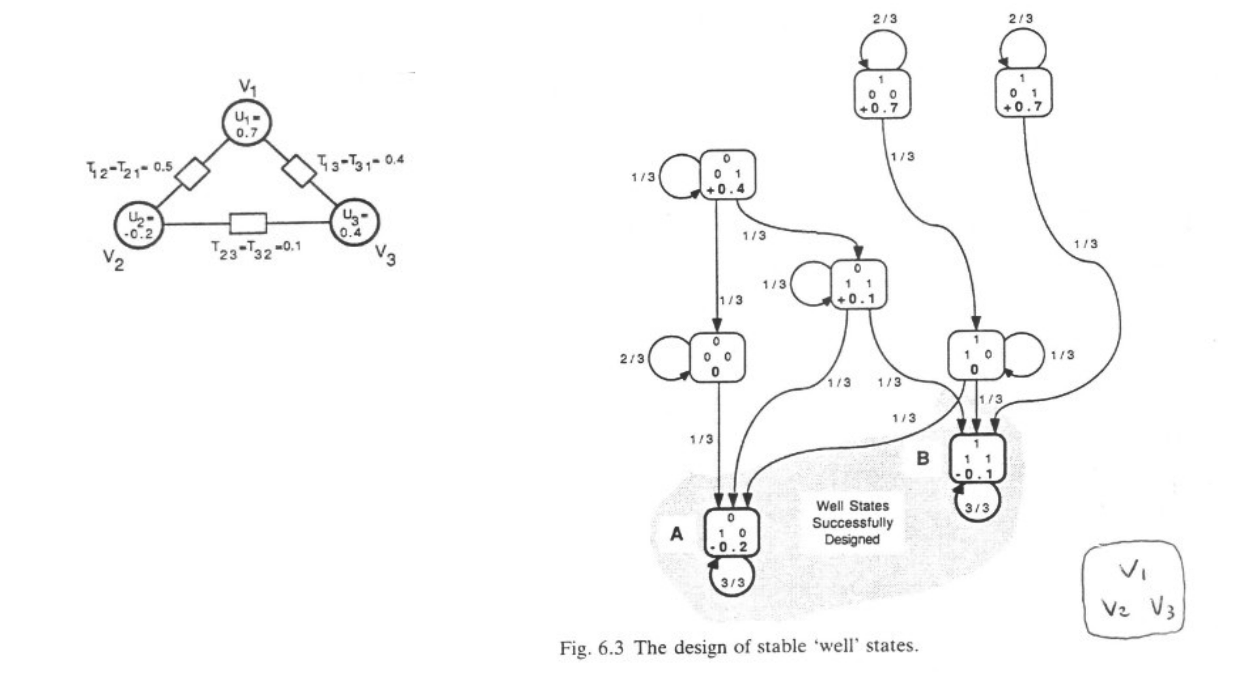
\includegraphics[ width=1.2\linewidth, height=\textheight, keepaspectratio]{./pics/reteHopfieldWellState.png}
    \caption{Reti di Hopfield, dove i neuroni al livello di energia più basso
    sono eletti \emph{stati stabili}.}
    \label{fig:reteHopfieldWellState}
\end{figure}



Tipicamente, per reti aventi $n$ neuroni è possibile eleggere $\log (n)$ stati
come stabili, esibendo dunque una crescita di tipo logaritmico.

Se si vuole imporre uno stato stabile, è necessario determinarlo con l'opportuna equazione. Supponiamo di voler imporre lo stato stabile $V_1 = 0$; per fare ciò, bisogna imporre $$T_{12} V_2 + T_{13} V_3 - U_1 < 0,$$ relativo al sistema di equazioni 


$$
\left\{
    \begin{array}{l}
    T_{12} - U_1 < 0 \\
    U_2 < 0 \\
    T_{23} - U_3 < 0
    \end{array}
\right.,
$$

che corrisponde all'imposizione dello stato stabile A in
Figura~\ref{fig:reteHopfieldWellState}. Sempre facendo riferimento alla stessa
rete, imporre lo stato stabile B significherebbe vedere soddisfatto il sistema
di equazioni

$$
\left\{
    \begin{array}{l}
        T_{12} + T_{13} - U_1 < 0 \\
        T_{12} + T_{23} - U_2 > 0 \\
        T_{23} + T_{13} - U_3 > 0 \\
    \end{array}
\right. .
$$

Infatti, avendo definito le quantità nella seguente maniera,

$$
\begin{array}{ll}
    T_{12} = T_{21} = 0,5 & U_1 = +0,7\\
    T_{13} = T_{31} = 0,4 & U_1 = -0,2\\
    T_{23} = T_{32} = 0,1 & U_1 = +0,4
\end{array}
$$

si ha che, per l'equazione di stato A (a sinistra), e l'equazione di stato B (a
destra)

$$
\left\{
    \begin{array}{llllll}
        0,5 - 0,7 < 0 & \leftrightarrow & \mbox{ Sì } & 0,5 + 0,4 - 0,7 > 0 & \leftrightarrow & \mbox{ Sì } \\
        -0,2  < 0 & \leftrightarrow & \mbox{ Sì } & 0,5 + 0,1 + 0,2 > 0 & \leftrightarrow & \mbox{ Sì } \\
        -0,1 - 0,4 < 0 & \leftrightarrow & \mbox{ Sì } & 0,1 + 0,4 - 0,4 > 0 & \leftrightarrow & \mbox{ Sì }
    \end{array}
\right.
$$

ed ambedue gli stati sono, di conseguenza, soddisfatti. In
Figura~\ref{fig:reteHopfieldWellState} essi corrispondono agli stati stabili
$010$ e $111$.

\subsection{La macchina di Boltzmann}

Può capitare che per una data rete di Hopfield vi siano alcuni minimi locali,
detti anche \emph{falsi minimi}; come ad esempio mostrato in
Figura~\ref{fig:retiMinimiLocali}; la soluzione corrispondente al minimo
globale potrebbe quindi non corrispondere a quella trovata mediante
l'evoluzione, se la rete è incappata in un minimo locale. Ciascun minimo locale
è, di fatto, uno stato stabile, dal quale nel caso vi si incappasse, non si
potrebbe uscire, poiché il livello di energia non può mai aumentare. 

Di solito,
si desidera che l'evoluzione converga verso gli stati stabili scelti, oppure
verso un minimo globale \---- i minimi locali, tuttavia, risulterebbero essere
alla stregua di ``falsi'' stati stabili, che andrebbero a minare il
comportamento desiderato della rete, per il quale sarebbe desiderabile ottenere
una soluzione unica, e corrispondente al minimo globale (o comunque a stati
stabili dal valore sufficientemente basso di energia). 

\begin{figure}[h]
    \centering
    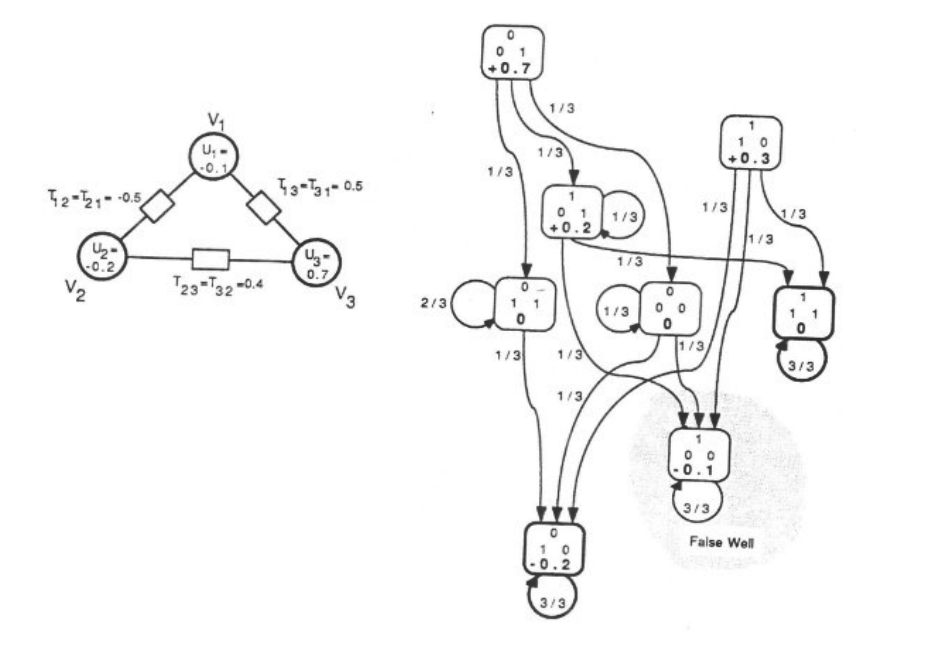
\includegraphics[ width=1.2\linewidth, height=\textheight, keepaspectratio]{./pics/retiMinimiLocali.png}
    \caption{Il problema dei \emph{falsi minimi}, anche detti minimi locali.}
    \label{fig:retiMinimiLocali}
\end{figure}



Con un po' di fortuna, i minimi locali possono avere un valore prossimo al
minimo assoluto; tuttavia ciò non è per nulla garantito, e non esistono criteri
matematici per stabilire la qualità della soluzione ottenuta. In altre parole,
\emph{non possiamo sapere a priori se la qualità della soluzione ottenuta},
incappando in uno stato stabile artificiale o di minimo locale, \emph{è
sufficientemente buona oppure non lo è.} 

Ciò rappresenta in ultima analisi un evidente difetto delle reti neurali di
Hopfield, poiché diversamente al paradigma della computazione procedurale dove
è sempre e comunque possibile ricondursi in qualche maniera al modello di
Turing o al modello RAM, e dunque ai teoremi studiati in tale ambito, nel
modello di computazione delle reti di Hopfield non c'è alcun criterio
matematico in grado di stabilire \textbf{a priori} la qualità di una
determinata soluzione.

Una soluzione al problema dei minimi locali imprevisti arrivò a cavallo degli
anni $80$, quando si cercò di superare il problema evocando la cosiddetta
\textbf{Boltzmann machine}, un modello della rete di Hopfield dove uno stato può
vedere \emph{aumentata la propria energia secondo una legge probabilistica},
violando dunque l'assunzione di base tale per cui l'energia complessiva della
rete può soltanto diminuire. Ciò viene attuato riscaldando in maniera
\emph{probabilistica} la rete, introducendo cioè una funzione \emph{sigmoidale}
dipendente da un parametro $T$, detto \emph{temperatura del neurone}; le
funzioni sigmoidali della macchina di Boltzmann sono progettate in modo tale
che una temperatura più elevata corrisponda a sigmoidi meno rigide, e
temperature che tendono allo $0$ termico corrispondono a sigmoidi molto simili
al tradizionale gradino.

Dunque, con il modello della macchina di Boltzmann,
temperature della rete molto basse e prossime allo zero termico produrrebbero
un comportamento della rete di Hopfield del tutto simile a quanto incontrato
sino ad ora, cioè ad un'evoluzione nella quale non sono ammessi aumenti del
livello dell'energia \---- viceversa, ad alte temperature del neurone si
assiste mano a mano a potenziali fenomeni in cui, al passaggio successivo, la
rete si è evoluta verso uno stato avente una maggiore energia rispetto a quello
precedente. L'idea di base della macchina di Boltzmann è quella di poter
``sfuggire'' all'attrazione dovuta ai minimi locali, introducendo la
possibilità probabilistica di poter ``tornare indietro'' e tentare una strada
evolutiva differente. La probabilità con cui un determinato stato possa
sfuggire dal minimo locale in cui risiede dipende dalla temperatura $T$ \-- più
essa è alta, maggiore sarà la probabilità per lo stato di aumentare la propria
energia e percorrere un'evoluzione differente.

\begin{figure}[h]
    \centering
    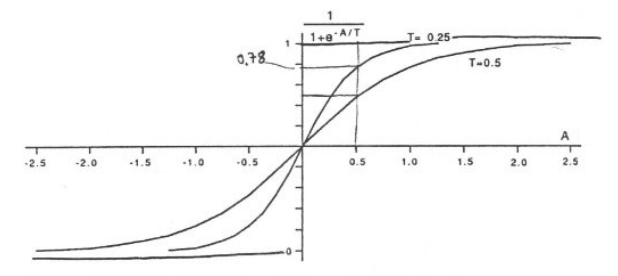
\includegraphics[ width=1.0\linewidth, height=\textheight, keepaspectratio]{./pics/boltzmannMachine.png}
    \caption{La funzione di attivazione probabilistica, con la sua tipica forma
    ``ad esse'' e comportamento dipendente dalla temperatura $T$. La sua forma
sarà tanto più simile al gradino ideale quanto la sua temperatura sarà tendente
allo $0$.}
    \label{fig:boltzmannMachine}
\end{figure}



Supponendo di disporre di un valore di attivazione $A = \sum_{j\neq i} T_{ij}
V_j - U_i$ pari a $ A = +0.5$, e una temperatura di $T=0,25$, avremo che la
probabilità di eccitazione del neurone sarà pari a $0,78$ invece che pari ad
$1$, come espresso in Figura~\ref{fig:boltzmannMachine}. Dunque, si dà la
possibilità al neurone di \emph{risalire la china dell'energia}, violando il
comportamento originale che invece aveva nella rete di Hopfield \-- con questo
stratagemma, la rete può probabilisticamente ``scappare'' dagli stati di minimo
locali non desiderati. Si aggiungono dunque nuovi percorsi che con una certa
probabilità dipendente dalla temperatura $T$ \emph{aumentano l'energia
della rete}: valori più alti di temperatura garantiscono una maggiore
probabilità di aumento dell'energia. 

Questo procedimento è chiamato \textbf{simulated annealing}, termine tratto
dalla metallurgia (ricottura), dove variazioni di temperatura di un materiale
sono adoperate per ottenere determinate caratteristiche dal materiale in
questione. La Figura~\ref{fig:retiBoltzmannMachine} illustra un esempio di rete
dove esiste una possibilità di ``risalire la china'', o più precisamente c'è
una probabilità non nulla di ritornare ad un livello di energia superiore.

\begin{figure}[h]
    \centering
    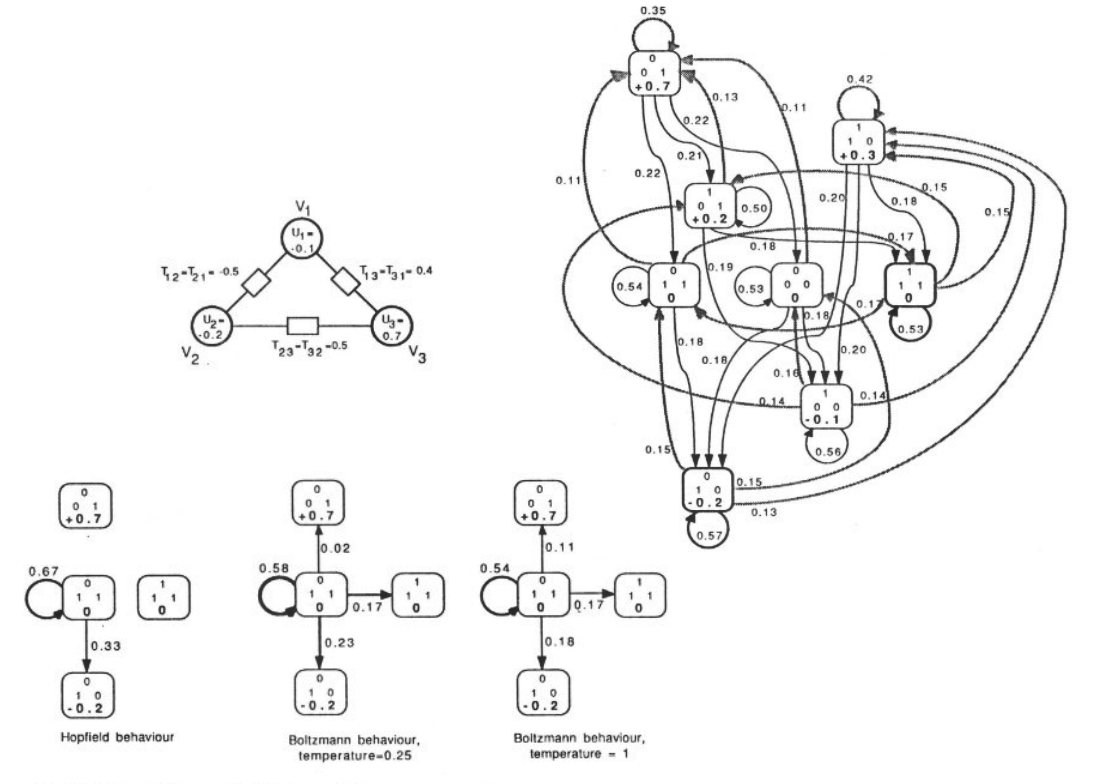
\includegraphics[ width=1.3\linewidth, height=\textheight, keepaspectratio]{./pics/retiBoltzmannMachine.png}
    \caption{Probabilità di transizione a differenti temperature $T$ (in
    basso); rete di Hopfield con estensione a macchina di Bolztmann (sopra).}
    \label{fig:retiBoltzmannMachine}
\end{figure}


E dunque grazie allo stratagemma della macchina di Boltzmann è possibile
progettare una rete di Hopfield che sia quantomeno robusta al problema dei
minimi locali, introducendo di fatto una sorta di \emph{perturbazione} alla
funzione di attivazione, che rende concretamente e probabilisticamente
possibile percorrere strade nuove e che consentono alla rete di ``fuoriuscire''
dalla situazione di stallo causata dallo stato di minimo locale in cui si
troverebbe imprigionata.


\section{La rete continua di Hopfield}

\begin{figure}[h]
    \centering
    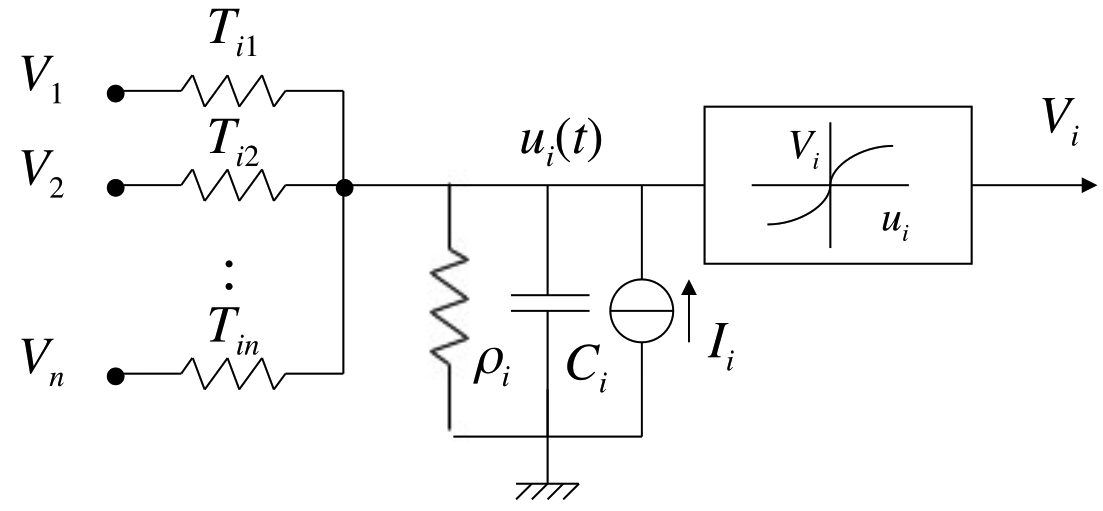
\includegraphics[ width=1.0\linewidth, height=\textheight, keepaspectratio]{./pics/reteHopfieldContinua.png}
    \caption{La \emph{rete continua di Hopfield}.}
    \label{fig:reteHopfieldContinua}
\end{figure}



La \textbf{rete continua di Hopfield} rappresenta un cambio di paradigma: mentre
prima la verifica sullo stato veniva fatto in tempi discreti, assumendo una
certa probabilità di interrogazione di un neurone, nella rete continua ogni
neurone è, con continuità, connesso ad ogni altro neurone e la verifica della
loro coerenza avviene istante per istante, mediante un \emph{circuito
analogico}. 

L'idea quindi è quella di lasciar evolvere il sistema composto dalla rete
neurale, facendo sì che le grandezze elettriche in questione sviluppino il loro
transitorio completamente: il risultato finale sarà la rete a minor energia.

Il valore d'uscita dipende da una funzione sigmoidale, ad esempio
$$V_i = g_i(u_i(t)) = \tanh (\frac{u_i(t)}{u_0}).$$ Alle conduttanze
d'ingresso, viene aggiunto un gruppo circuitale
resistenza-condensatore-generatore di corrente che produce correnti
parallelamente a quelle di ingresso, cioè che si somma a quelle di ingresso.
La totale conduttanza di neurone sarà pari a

$$ \frac{1}{R_i} = \frac{1}{\rho_i} + \sum_j \frac{1}{R_j}, $$

e tramite le leggi di Norton, si ottiene l'equazione del neurone,

\begin{equation}\nonumber
    \sum_j (V_j - u_j(t)) T_{ij} + I_i = C_i \frac{du_i(t)}{dt} + \frac{u_i(t)}{\rho_i}
\end{equation}

mentre l'energia della rete sarà


\begin{equation}
    E = -\frac 1 2 \sum{ij, j\neq i} T_{ij} V_i V_j + \sum_i \frac{1}{R_i}
    \int_0^{V_i} g_i^{-1} (V) dV - \sum_i I_i V_i.
\end{equation}

Calcolando la variazione dell'energia, 

$$ \frac{dE}{dt} = \sum_i \frac{dE}{dV_i} \frac{dV_i}{dt},$$ pertanto si avrà che

\begin{eqnarray}\nonumber
    \frac{dE}{dV_i} & = & -\sum_j T_{ij}V_j + \frac{u_i}{R_i} - I_i = -C_i\frac{du_i}{dt} \\\nonumber
    \frac{dE}{dt}   & = & -\sum_i \left(\sum_j T_{ij}V_j + \frac{u_i}{R_i} - I_i\right)\frac{dV_i}{dt} = -\sum_i C_i\frac{du_i}{dt}\frac{dV_i}{dt} \\\nonumber
                    & = & -\sum_i C_i(\frac{du_i}{dV_i})\left(\frac{dV_i}{dt}\right)^2 \\\nonumber
                    & = & -\sum_i g_i^{-1}(V_i)C_i\left(\frac{dV_i}{dt}\right)^2 \leq 0,
\end{eqnarray}

dove si è osservato che $g_i^{-1}(V_i) > 0, \forall V_i$ poiché monotona
crescente. In definitiva la variazione netta di energia della rete sarà

\begin{equation}
    \frac{dE}{dt} \leq 0,
\end{equation}

con l'uguaglianza a zero rispettata solo ed esclusivamente nel caso in cui
$\displaystyle \frac{dV_i}{dt} = 0, \forall i$. Dunque, anche nel caso della
rete continua di Hopfield la variazione di energia sarà sempre negativa.

In ultima analisi, \emph{il tempo di risposta} di una rete di Hopfield dipende
esclusivamente dalla costante di tempo $\tau$ del neurone, poiché per ottenere
una soluzione è necessario che il transitorio dell'evoluzione della rete abbia
termine. Di fatto, il tempo di risposta non dipende dalla complessità della
rete, bensì unicamente dalla costante di tempo \-- diversamente per quanto
accadeva con le reti discrete di Hopfield.

Degno di nota è il fatto che il rapporto ingresso-uscita è fissato da una
sigmoide, non è garantito che il valore d'uscita sia ad un valore nettamente
basso o nettamente alto, cioè non è garantito un perfetto comportamento a
soglia. Esistono infatti valori in concomitanza con lo $0$ d'ingresso che
possono suscitare dubbi interpretativi, cioè il neurone potrebbe collocarsi ad
un valore intermedio fra valore alto e basso. 


\section{Soluzione dei problemi con la rete di Hopfield}

Con una rete di Hopfield si può risolvere un problema solo se esso può essere
codificato nei termini della \emph{minimazione di una forma quadratica}. La
soluzione sarà \emph{ottima} se l'energia ottenuta è quella corrispondente al
minimo assoluto \---- viceversa, sarà \emph{sub-ottimale} se l'energia ottenuta
corrisponderà invece a quella di un minimo locale, o comunque di uno stato
stabile vero o falso che sia ad energia maggiore di quella fornita dal minimo
globale.

La strategia è la seguente: individuata la forma quadratica associata al
problema, per confronto si ricavano i valori $T_{ij}$ ed $I_i$ che consentono
la costruzione della rete. Successivamente, la rete è lasciata evolvere; la
soluzione corrispondente viene prelevata e il problema viene risolto con la
soluzione ricavata mediante la codifica.

\subsection{Il problema della memoria indirizzabile}

Si desidera che $V^s(s=1,2,\dots, n)$ siano stati stabili in una rete dotata di
$n$ neuroni. 

La quantità da minimizzare sarà $E^* = -\frac 1 2 \sum_s (V^s\cdot
V)^2$, con $V=V^s$ valore negativo di energia minimo: ciò accade poiché siamo
di fronte ad un prodotto scalare che massimizza la quantità all'interno della
sommatoria, con il risultato di minimizzare il valore dell'energia. 

Se $V$ è
casuale e $(-1 \leq V_i \leq +1)$, la $E^*$ risulterà essere circa nulla \--
eseguendo un prodotto scalare fra due vettori sostanzialmente molto differenti;
il valore minimo si raggiunge con $V=V^s$, ed è tale che $E^* = -\frac 1 2
n^2$. 

Bisogna in pratica fissare anticipatamente i $V^s$ di stato stabile, e
con essi si ottiene $$ E = -\frac 1 2 \sum_s (V^s V)^2 = \dots = -\frac 1 2
\sum_i \sum_j (\sum_s V_i^s V_j^s)V_i V_j,$$ ma sappiamo anche che

$$E= -\frac 1 2 \sum_{ij} T_{ij}V_i V_j - \sum_i I_i V_i.$$ Dal confronto fra
le due equazioni è presto ricavato che 

$$
\left\{
    \begin{array}{lll}
        T_{ij} & = & \sum_s V_i^s V_j^s \\
        I_i & = & 0
    \end{array}
\right.
$$

cioè abbiamo trovato (?)





\end{document}
